%%
%% Plantilla elsarticle (Elsevier), citas autor-año.
%% En el texto: \citet{clave} -> Autor (año); \citep{clave} -> (Autor, año).
%% Compilar: pdflatex articulo -> bibtex articulo -> pdflatex articulo (x2)
%%
%% Las imágenes van en la carpeta figuras/ (ver \graphicspath más abajo).
%%

\documentclass[preprint,12pt,authoryear]{elsarticle}

\usepackage[T1]{fontenc}
\usepackage[spanish,es-nodecimaldot,es-tabla]{babel}
\usepackage{amssymb}
\usepackage{amsmath}
\usepackage{xcolor}
\usepackage{xurl}      % permite cortar URL largas en las referencias

%% ---- Imágenes ----
\usepackage{graphicx}          % da el comando \includegraphics
\graphicspath{{figuras/}}      % carpeta donde LaTeX busca las imágenes

%% ---- Tablas ----
\usepackage{booktabs}          % líneas \toprule, \midrule, \bottomrule
\usepackage{array}
\usepackage{xltabular}         % tablas que se parten entre páginas (incluye tabularx)
\newcolumntype{L}{>{\raggedright\arraybackslash}X}          % columna flexible
\newcolumntype{P}[1]{>{\raggedright\arraybackslash}p{#1}}   % columna de ancho fijo
\newcolumntype{C}[1]{>{\centering\arraybackslash}p{#1}}     % columna centrada

%% ---- Diagramas dibujados en LaTeX (mapa del problema) ----
\usepackage{tikz}
\usetikzlibrary{positioning,arrows.meta,fit,backgrounds,babel}
\newcommand{\titulocaja}{\footnotesize\bfseries}  % títulos de las cajas del mapa

\usepackage[hidelinks]{hyperref}

%% Títulos en español para el resumen y las palabras clave
\abstracttitle{Resumen}
\keywordtitle{Palabras clave}

%% Marca para lo que falta llenar cuando estén los resultados de escenarios
\newcommand{\pendiente}[1]{\textcolor{red}{[PENDIENTE: #1]}}

%% PROVISIONAL: definir la revista. Opciones afines al tema: Agricultural Systems,
%% Food Policy, Journal of Agriculture and Food Research, Simulation Modelling
%% Practice and Theory.
\journal{Agricultural Systems}

\begin{document}

\begin{frontmatter}

%% Título original del borrador:
%% \title{Dinámica de sistemas aplicada a la gestión de inventarios y
%% producción avícola ante fluctuaciones macroeconómicas}
\title{Ciclo de oferta y precio del huevo en Colombia: un modelo de dinámica de sistemas para evaluar políticas de estabilización}

%% Revisar la lista de autores (en los comentarios del borrador aparecen
%% también Sebastián y Camilo) y quién es el autor de correspondencia.
\author{Johan Portilla}
\author{Diego Muñoz}
\author{Juan Velasco}
\author{Joan Aguirre}
\author{Oscar Rubiano\corref{cor1}}
\cortext[cor1]{Autor de correspondencia.}

\affiliation{organization={Escuela de Ingeniería Industrial, Universidad del Valle},
            city={Santiago de Cali},
            country={Colombia}}

\begin{abstract}
Entre 2019 y 2026 el mercado colombiano del huevo pasó por fases de escasez con precios altos y de sobreoferta con márgenes negativos, que en enero de 2026 llevaron a los avicultores a protestar y a pedir la regulación del encasetamiento y un fondo de estabilización de precios. Este artículo explica ese ciclo y evalúa políticas para atenuarlo con un modelo de dinámica de sistemas de paso semanal que va de 2019 a 2030. El modelo representa como niveles las pollitas en levante y las gallinas en postura, e incluye una regla de encasetamiento de anclaje y ajuste que cuenta solo en parte las aves que ya vienen en camino, un precio mayorista endógeno, la entrada de productores por imitación, la capacidad de los galpones y la caja del productor. Se calibró con series semanales del gremio avícola, precios mayoristas oficiales y censos pecuarios de 2019 a 2025, y el año 2026 se reservó como prueba fuera de muestra. El modelo reproduce el encasetamiento con un error porcentual absoluto medio de 5,9~\%, la producción con 2,9~\% y el precio mayorista con 7,1~\%; en 2026 el error del precio es de 3,6~\%. La calibración indica decisiones lentas: el productor percibe el precio con unas 26 semanas de rezago y cierra la brecha de su hato de gallinas en cerca de dos años. \pendiente{resultados de los escenarios de cuota de encasetamiento, fondo de compra de excedentes, información completa y vida productiva extendida, medidos con la variabilidad del precio real, las semanas con margen negativo, la salida de productores y el consumo por persona.} \pendiente{conclusión principal.}

\medskip
\noindent\textbf{Abstract.} Between 2019 and 2026, the Colombian egg market alternated between scarcity with high prices and oversupply with negative margins; in January 2026 producers protested and asked the government to regulate chick placements and to create a price stabilisation fund. This paper explains the cycle and assesses policies to dampen it with a weekly system dynamics model covering 2019--2030. Pullets in rearing and laying hens are modelled as stocks. Placements follow an anchoring-and-adjustment rule that only partly accounts for birds already in the supply line, the wholesale price is endogenous, new producers enter by imitation, and housing capacity and producer cash are tracked explicitly. The model was calibrated with weekly industry data, official wholesale prices and livestock census records for 2019--2025 and tested out of sample on 2026. It reproduces chick placements with a mean absolute percentage error of 5.9\%, egg output with 2.9\% and the wholesale price with 7.1\%; the out-of-sample price error for 2026 is 3.6\%. The calibrated decision rule is slow: producers perceive prices with a lag of about 26 weeks and close the gap in their laying flock over roughly two years. \pendiente{scenario results.} \pendiente{main conclusion.}

\smallskip
\noindent\textit{Keywords:} system dynamics; commodity cycle; table eggs; chick placement; supply line; price stabilisation; Colombia.
\end{abstract}

%% Graphical abstract (opcional en la mayoría de revistas Elsevier)
%% \begin{graphicalabstract}
%% \includegraphics{grabs}
%% \end{graphicalabstract}

%% Highlights: de 3 a 5, máximo 85 caracteres cada uno (con espacios).
\begin{highlights}
\item Modelo de dinámica de sistemas del ciclo de oferta y precio del huevo en Colombia
\item Calibrado con datos semanales del gremio, precios oficiales y censos, 2019-2025
\item Reproduce encasetamiento y precio con errores medios de 5,9 \% y 7,1 \%
\item Compara cuota de encasetamiento, fondo de estabilización e información completa
\item Las políticas se miden con indicadores del productor y del consumidor a 2030
\end{highlights}

\begin{keyword}
dinámica de sistemas \sep ciclo de commodities \sep huevo \sep encasetamiento \sep línea de suministro \sep estabilización de precios \sep Colombia
\end{keyword}

\end{frontmatter}

%% ===================================================================
\section{Introducción}
\label{sec1}

El huevo es un alimento denso en nutrientes, que mejora el crecimiento infantil \citep{Iannotti2017}, y una de las proteínas animales de menor costo para los hogares. En Colombia su consumo creció con rapidez: según la Federación Nacional de Avicultores de Colombia (Fenavi), el país produjo 19.402 millones de huevos en 2025 y el consumo aparente llegó a 366 unidades por persona al año, frente a unas 291 en 2019 \citep{Fenavi2026Estadisticas,Fenavi2026Fenaviquin440,Quintero2026}. Esa oferta se decide muchos meses antes de llegar al mercado. El gremio llama encasetamiento al ingreso de pollitas de un día a las granjas de postura; las aves pasan unas 20 semanas en levante y después producen durante cerca de 60 \citep{Fenavi2026Fenaviquin440}. Lo que un productor encaseta hoy fija buena parte de la oferta del año y medio siguiente, y lo decide sin conocer el precio que encontrará cuando sus aves empiecen a poner.

%% Cambio del 18-nov: las caídas del precio son las cifras reales que calculó
%% el grupo con SIPSA e IPC (las mismas de la sección 3). Antes decía, con
%% Fenaviquín 440: "cayó 18,2 % en 2024 y 5,8 % en 2025" (precio nominal).
Entre 2019 y 2026 ese rezago se tradujo en un ciclo marcado. El encasetamiento cayó en 2021, la producción se contrajo en 2022 y el precio mayorista que registra el Departamento Administrativo Nacional de Estadística (DANE) alcanzó sus máximos en 2022 y 2023 \citep{Fenavi2026Estadisticas,DANE2026SIPSA}. Esa rentabilidad atrajo más aves y más productores: el encasetamiento pasó de 45,3 millones de pollitas en 2021 a 58,3 millones en 2025 \citep{Fenavi2026Estadisticas}, y el precio mayorista real bajó 16,4~\% en 2024 y 9,7~\% en 2025 \citep{DANE2026IPC,DANE2026SIPSA}. En enero de 2026 los productores protestaron para pedir que se regulara el encasetamiento y se creara un fondo de estabilización de precios \citep{Villamizar2026}, y entre enero y julio el encasetamiento fue cerca de 12~\% menor que un año antes \citep{Quintero2026}, lo que anticipa una nueva fase de menor oferta. En cada vuelta del ciclo pierden los avicultores durante la sobreoferta y los hogares durante la escasez.

Este comportamiento es el de los ciclos de producción de los mercados pecuarios. Surgen cuando la oferta responde con rezago al precio \citep{Ezekiel1938}, y la dinámica de sistemas los explica por las demoras en la percepción del precio, en la decisión de invertir y en la producción biológica \citep{Meadows1969}. La evidencia experimental añade por qué los decisores sobrecorrigen: al decidir cuánto pedir cuentan, en promedio, cerca de un tercio de lo que ya viene en camino \citep{Sterman1989b}. El mercado del huevo reúne esas condiciones, y la dinámica de sistemas ya se ha usado para reproducir ciclos y comparar políticas en cadenas avícolas, sobre todo en Indonesia \citep{Yuzaria2025,Haryana2026}.

En Colombia, en cambio, el mercado del huevo se ha estudiado con métodos econométricos y descriptivos \citep{EcheverrySilva2009,RodriguezTorres2020}, y los modelos de dinámica de sistemas del agro tratan otras cadenas o la escala de la granja \citep{AnaconaMopan2023,ParraOrtega2025}. En la revisión de la literatura (sección~\ref{sec2}) no encontramos un modelo del ciclo nacional del huevo, ni uno que reúna la línea de suministro con un peso explícito en la decisión, la entrada de productores atraídos por la rentabilidad y los galpones como costo hundido, o que evalúe las medidas que hoy piden los avicultores.

Este artículo desarrolla y calibra un modelo de dinámica de sistemas del ciclo del huevo de mesa en Colombia, con paso semanal entre 2019 y 2030, con dos propósitos. El primero es explicar cómo el rezago biológico, la regla de encasetamiento y la entrada de productores generaron las oscilaciones de producción y precio de 2019 a 2026. El segundo es comparar, con indicadores del productor y del consumidor, cuatro políticas: una cuota de encasetamiento, un fondo que compra excedentes cuando el precio cae por debajo del costo, la publicación oportuna del encasetamiento para que cada productor cuente las aves que vienen en camino y la extensión de la vida productiva de las gallinas. El modelo se calibró con datos de Fenavi, del Sistema de Información de Precios y Abastecimiento del Sector Agropecuario (SIPSA) del DANE y de los censos pecuarios del Instituto Colombiano Agropecuario (ICA), y se probó fuera de muestra con los de 2026. Es un modelo explicativo, construido para comparar políticas y no para pronosticar precios. Sus aportes son tres: una estructura del ciclo del huevo calibrada con datos colombianos, una estimación de la lentitud con que los productores perciben el precio y ajustan su hato, y una comparación de políticas que mide también su efecto sobre los hogares.

La sección~\ref{sec2} revisa la literatura y la sección~\ref{sec3} presenta los materiales y métodos. La sección~4 analiza la corrida base, la dominancia de los bucles y los escenarios; la sección~5 discute los resultados y la sección~6 presenta las conclusiones.

%% ===================================================================
\section{Revisión de literatura}
\label{sec2}

\subsection{Método de la revisión}
\label{sec2.1}

Se hizo una revisión narrativa con protocolo explícito, guiada por cuatro preguntas: qué explica los ciclos de producción y de precio en los mercados pecuarios con demoras biológicas (PR1); cómo deciden los productores cuando parte de la producción ya está en camino, es decir, cuando hay una línea de suministro (PR2); qué modelos de dinámica de sistemas existen para cadenas pecuarias, avícolas y del huevo, y qué políticas evalúan (PR3); y qué se sabe del mercado del huevo y de las políticas de estabilización que sea útil para el caso colombiano (PR4).

Las búsquedas se hicieron en octubre de 2026, en inglés y en español, en Scopus, Google Scholar, \textit{System Dynamics Review}, RePEc, AgEcon Search, SciELO, Redalyc, Dialnet y los repositorios de tesis del Massachusetts Institute of Technology (MIT), Curtin University y la University of Manitoba. Los términos combinaron, entre otros, \textit{system dynamics} con \textit{poultry} o \textit{egg}; \textit{commodity cycle} o \textit{cobweb} con \textit{lag}; \textit{supply line} o \textit{misperception of feedback}; \textit{egg price} con \textit{avian influenza} o \textit{supply management}; y \textit{dinámica de sistemas} con \textit{avícola} o \textit{huevo}. Se incluyeron artículos y tesis en inglés o en español que respondieran al menos una pregunta y tuvieran una referencia verificable (DOI o registro en un repositorio), sin límite de fecha para no perder los trabajos clásicos. Se excluyeron los informes gremiales, los boletines estadísticos y las notas de prensa, que el artículo usa como fuentes de datos, y los libros de texto del marco metodológico, como \citet{Sterman2000}. Cada documento se registró en una matriz con su método, su hallazgo principal y su uso en este artículo (Anexo~A).
%% PENDIENTE: agregar el Anexo A con las ecuaciones de búsqueda y la matriz
%% (Tabla A1 de Revision_literatura_huevo.docx), con las filas de Lu (2020),
%% Atzori et al. (2023) y Parra-Ortega et al. (2025).

El corpus final tiene 32 documentos, 28 artículos y 4 tesis, publicados entre 1938 y 2026; seis tratan casos colombianos y cuatro están en español. La Tabla~\ref{tab:corpus} los agrupa en los cuatro temas que organizan la sección.

\begin{table}[!htbp]
\centering
\caption{Documentos revisados por tema.}
\label{tab:corpus}
\footnotesize
\setlength{\tabcolsep}{4pt}
\begin{tabularx}{\textwidth}{@{}P{3.3cm}C{1.2cm}LC{0.8cm}@{}}
\toprule
Tema & Pregunta & Documentos & Total \\
\midrule
A. Ciclos de producción en los mercados pecuarios & PR1 & \citet{Ezekiel1938}; \citet{Nerlove1958}; \citet{Harlow1960}; \citet{Meadows1969}; \citet{Fisher1974}; \citet{Rosen1994}; \citet{Chavas1999}; \citet{BergHuffaker2015} & 8 \\
\addlinespace
B. Decisiones con demoras y línea de suministro & PR2 & \citet{Sterman1989a}; \citet{Sterman1989b}; \citet{Kampmann1992}; \citet{CrosonDonohue2006}; \citet{ArangoMoxnes2012}; \citet{KampmannSterman2014} & 6 \\
\addlinespace
C. Dinámica de sistemas en cadenas pecuarias, avícolas y agrícolas & PR3 & \citet{MinegishiThiel2000}; \citet{VoThiel2011}; \citet{Shamsuddoha2014}; \citet{Dizyee2017}; \citet{Lu2020}; \citet{RubianoIbarraVega2021}; \citet{Atzori2023}; \citet{AnaconaMopan2023}; \citet{ParraOrtega2025}; \citet{Saepullah2025}; \citet{Yuzaria2025}; \citet{Haryana2026} & 12 \\
\addlinespace
D. Mercado del huevo y políticas de estabilización & PR4 & \citet{EcheverrySilva2009}; \citet{Cardwell2015}; \citet{AlonsoCifuentes2017}; \citet{RodriguezTorres2020}; \citet{TraoreDoyon2023}; \citet{Mitchell2024} & 6 \\
\midrule
Total & & & 32 \\
\bottomrule
\end{tabularx}

\smallskip
{\footnotesize\raggedright Fuente: elaboración propia.\par}
\end{table}

\subsection{Ciclos de producción en los mercados pecuarios}
\label{sec2.2}

El teorema de la telaraña es la explicación clásica: si los productores deciden cuánto producir con el precio actual y la producción tarda un periodo en salir, el precio y la cantidad se alternan entre valores altos y bajos, y la oscilación se amortigua, se mantiene o crece según las pendientes de la oferta y la demanda \citep{Ezekiel1938}. Con expectativas adaptativas, que se acercan poco a poco al precio observado, el mercado es más estable \citep{Nerlove1958}. \citet{Harlow1960} encontró en el cerdo un ciclo de unos cuatro años, el doble del que predecía la versión simple, y lo atribuyó a rasgos de la producción porcina: la duración del ciclo depende de la longitud de las demoras biológicas.

\citet{Meadows1969} llevó la telaraña a la dinámica de sistemas. Su «teorema dinámico de la telaraña» explica los ciclos del cerdo, el ganado y el pollo por las demoras en la percepción del precio, en la decisión de invertir y en la producción biológica, y es el antecedente directo de este modelo. \citet{Fisher1974} comparó mínimos cuadrados en dos etapas, regresión múltiple y un modelo de dinámica de sistemas del ciclo del cerdo, y ninguno pronosticó bien el sector; de ahí que el modelo del huevo se use para explicar el ciclo y comparar políticas.

El ciclo persiste aun con productores informados. En el ganado, el hato es a la vez capital y producto, y su estructura de edades basta para generar ciclos con expectativas racionales \citep{Rosen1994}; las pollitas en levante y las gallinas en postura forman una estructura parecida. Cerca del 73~\% de los participantes del mercado porcino de Estados Unidos forma sus expectativas con precios pasados \citep{Chavas1999}, y en Alemania el ciclo del cerdo se sostiene por la baja elasticidad de la demanda, la irreversibilidad de la inversión en instalaciones y una inversión que depende de la liquidez de los productores \citep{BergHuffaker2015}.

\subsection{Decisiones con demoras y línea de suministro}
\label{sec2.3}

\citet{Sterman1989b} estimó, con el juego de la cerveza, la regla con que los participantes hacen sus pedidos: parten de la demanda esperada y corrigen la brecha entre el inventario deseado y el real y la brecha entre los pedidos en camino deseados y los reales. En promedio, dieron a los pedidos en camino un peso de 0,34, el valor de referencia del modelo. Al ignorar cerca de dos tercios de la línea de suministro, piden de más cuando falta inventario y de menos cuando sobra, y el sistema oscila. Un experimento de inversión de capital llevó a la misma conclusión \citep{Sterman1989a}, y la regla de encasetamiento del modelo tiene esa forma.

Los experimentos posteriores matizan el resultado. El efecto látigo persiste aun cuando los participantes conocen la distribución de la demanda, y compartir la información de inventario lo reduce \citep{CrosonDonohue2006}; ese hallazgo sostiene el escenario de información completa. Los mercados con formación de precios moderan la mala percepción de la realimentación, pero no la eliminan, y las reglas de decisión estimadas, de racionalidad limitada, reproducen la dinámica observada \citep{Kampmann1992,KampmannSterman2014}. En el experimento de la telaraña de \citet{ArangoMoxnes2012}, los ciclos aparecieron al agregar demoras de inversión y generaciones de capacidad, porque los participantes daban poco peso a la capacidad en construcción. El sector del huevo reúne ambas condiciones: un levante de unas 20 semanas y lotes de aves de distintas edades que producen al mismo tiempo.

\subsection{Dinámica de sistemas en cadenas pecuarias y avícolas}
\label{sec2.4}

La dinámica de sistemas se usa en cadenas agroalimentarias desde hace más de dos décadas. \citet{MinegishiThiel2000} la aplicaron a una cadena integrada de pollo en Francia, y \citet{VoThiel2011} compararon políticas de flexibilidad, inventario, reserva y suavización en la cadena francesa del pollo durante una crisis de influenza aviar. \citet{Shamsuddoha2014} modeló la cadena avícola de Bangladés, y \citet{Dizyee2017} unieron la biología del hato, el mercado y los choques sanitarios de la carne bovina de Botsuana, donde la mejor política combinó la liberalización de las exportaciones con el control de enfermedades. \citet{Lu2020} probaron estrategias contracíclicas en el ciclo del cerdo, y \citet{Atzori2023} representaron un hato lechero con una cadena de envejecimiento calibrada con registros de finca, la estructura con que aquí se representan las aves.

Los antecedentes más cercanos al huevo son de Indonesia. En el modelo de gallinas ponedoras de \citet{Yuzaria2025}, un bucle de balance hace que la sobreoferta baje el precio y uno de refuerzo convierte las ganancias en crédito y más aves; un alza anual de 60~\% en el costo del alimento reduce la producción cerca de 25~\% al año. \citet{Saepullah2025} identificaron en la cadena del huevo de Banten bucles de salud de las aves, de ajuste por precio y de restricción por costos. \citet{Haryana2026} mostraron que las oscilaciones del precio del pollo de engorde y los largos periodos de precio por debajo del costo nacen de la realimentación y de las demoras biológicas, y que ajustar la incubación es la palanca más fuerte a corto plazo, porque frena el excedente antes de que llegue al mercado. Es la evidencia más directa a favor de la cuota de encasetamiento.

En Colombia, \citet{AnaconaMopan2023} modelaron la cadena del aguacate Hass en el Cauca y encontraron que las estrategias combinadas de crédito, logística y apoyo técnico favorecen a los pequeños productores. \citet{RubianoIbarraVega2021} activaron las medidas de contención de un modelo epidemiológico SIR (susceptibles, infectados y recuperados) ampliado cuando los infectados superaban un umbral, la misma forma con que el modelo activa la cuota de encasetamiento. \citet{ParraOrtega2025} modelaron el efecto de los ciclos de producción de una granja de postura sobre su flujo de capital.

\subsection{El mercado del huevo y las políticas de estabilización}
\label{sec2.5}

Los estudios colombianos sobre el huevo son econométricos o descriptivos. En el Valle del Cauca, el precio al productor subió mucho menos que el precio al consumidor y los intermediarios se quedaron con la mayor parte del margen \citep{EcheverrySilva2009}; en Bogotá, el precio al consumidor responde más a las alzas del precio mayorista (0,219) que a las bajas (0,141), y la mitad del efecto tarda unos 7,5 meses en llegar \citep{RodriguezTorres2020}. El precio en granja, el mayorista y el del consumidor son, entonces, variables distintas que el modelo debe separar.

En otros países se subraya el peso de las existencias de aves. La influenza aviar de 2022 y 2023 subió el precio minorista del huevo en Estados Unidos cerca de 5,3~\%, y los modelos que ignoran la recuperación del inventario de ponedoras sobrestiman entre tres y cuatro veces las pérdidas de los consumidores \citep{Mitchell2024}. En granjas de Quebec, alargar el ciclo de postura de unas 51 a 64 semanas subió la utilidad cerca de 6~\% al año, y el óptimo económico estuvo en 71 semanas \citep{TraoreDoyon2023}: la vida productiva es una decisión del productor y no una constante biológica.

Sobre las políticas, la evidencia advierte de costos y de problemas de diseño. Las cuotas canadienses de lácteos y aves cuestan a los hogares más pobres cerca de 2,3~\% de su ingreso al año, frente a 0,5~\% a los más ricos \citep{Cardwell2015}, de modo que la cuota debe medirse también con indicadores del consumidor. En Colombia, el Fondo de Estabilización de Precios del Azúcar aisló los precios internos de los internacionales entre 2001 y 2015 \citep{AlonsoCifuentes2017}. Un fondo para el huevo, en cambio, tendría que enfrentar una sobreoferta generada dentro del sector, y por eso el escenario lo representa como una compra de excedentes cuando el precio cae por debajo del costo.

\subsection{Síntesis y brecha}
\label{sec2.6}

La revisión deja tres conclusiones: los ciclos pecuarios nacen de combinar demoras biológicas, expectativas adaptativas e inversiones difíciles de revertir \citep{Meadows1969,Rosen1994,BergHuffaker2015}; la regla que ignora la línea de suministro amplifica las oscilaciones, y la información la atenúa sin eliminarla \citep{Sterman1989b,CrosonDonohue2006,KampmannSterman2014}; y la dinámica de sistemas ya reproduce ciclos y evalúa políticas en cadenas avícolas \citep{VoThiel2011,Haryana2026}. Sin embargo, ninguno de los modelos revisados reúne en una misma estructura la línea de suministro con un peso explícito, la entrada de productores por imitación y el costo hundido de los galpones, ni evalúa las políticas que hoy se discuten en Colombia, donde no se encontró un modelo de dinámica de sistemas del ciclo del huevo. La Tabla~\ref{tab:aporte} resume qué toma el modelo de la literatura y qué le agrega.

\begin{table}[!htbp]
\centering
\caption{Aporte del modelo frente a la literatura revisada.}
\label{tab:aporte}
\footnotesize
\setlength{\tabcolsep}{4pt}
\begin{tabularx}{\textwidth}{@{}P{2.5cm}P{3.7cm}L@{}}
\toprule
Elemento del modelo & Antecedentes & Qué agrega este artículo \\
\midrule
Demora biológica de levante y postura & \citet{Meadows1969}; \citet{Rosen1994}; \citet{Haryana2026} & Pollitas en levante con una demora de tercer orden de 20 semanas y gallinas en postura en tres etapas, con parámetros de Fenavi. \\
\addlinespace
Precio endógeno y expectativas adaptativas & \citet{Ezekiel1938}; \citet{Nerlove1958}; \citet{Chavas1999} & Precio mayorista según la relación entre la demanda y la producción, y precio percibido suavizado, contrastados con el SIPSA. \\
\addlinespace
Línea de suministro subponderada & \citet{Sterman1989b}; \citet{CrosonDonohue2006}; \citet{ArangoMoxnes2012} & Peso explícito de las pollitas en camino en la regla de encasetamiento (0,34) y un escenario en que se cuentan todas. \\
\addlinespace
Entrada y salida de productores & En parte: expansión financiada con las ganancias \citep{Yuzaria2025} e inversión según la liquidez \citep{BergHuffaker2015} & Entrada por imitación según el margen, con la estructura del modelo de difusión, y salida cuando se agota la caja. \\
\addlinespace
Costo hundido de la capacidad & \citet{ArangoMoxnes2012}; \citet{BergHuffaker2015} & Capacidad de galpones como nivel: los cupos vacíos por encima de la holgura normal presionan el encasetamiento cuando el precio cae. \\
\addlinespace
Políticas de estabilización & \citet{Cardwell2015}; \citet{AlonsoCifuentes2017}; \citet{TraoreDoyon2023}; \citet{Haryana2026} & Cuota de encasetamiento, fondo de compra de excedentes, información completa y vida productiva extendida, comparadas entre 2027 y 2030 con indicadores del productor y de los hogares. \\
\addlinespace
Contexto & Casos de Francia, Bangladés, Botsuana, Indonesia y Estados Unidos, entre otros; estudios colombianos del huevo econométricos o descriptivos & Modelo del ciclo nacional del huevo en Colombia calibrado con datos de 2019 a 2025 y probado fuera de muestra con los de 2026. \\
\bottomrule
\end{tabularx}

\smallskip
{\footnotesize\raggedright Fuente: elaboración propia con base en los documentos citados.\par}
\end{table}

%% ===================================================================
\section{Materiales y métodos}
\label{sec3}

\subsection{Marco metodológico}
\label{sec3.1}

El estudio sigue el proceso de modelado de \citet{Sterman2000}, que va de la articulación del problema a la hipótesis dinámica, la formulación del modelo, las pruebas y el diseño y evaluación de políticas, y lo combina con el análisis funcional y estructural de \citet{RubianoVillarreal}, que lleva de los síntomas de un problema a un modelo de simulación y a la comparación de escenarios. El trabajo tuvo seis etapas:
\begin{enumerate}
\item formulación del problema con las cinco preguntas (qué, cuánto, cuándo, dónde y a quién afecta) y con la separación entre señales de resultados, señales de procesos y causas derivadas (sección~\ref{sec3.2});
\item descripción del sistema con un diagrama SIPOC (por sus siglas en inglés: proveedores, entradas, proceso, salidas y clientes) y un diagrama de flujos de materiales, información y decisiones al estilo de \citet{Hollingsworth1995} (sección~\ref{sec3.3});
\item construcción de una base de datos con series de 2017 a 2026 y medición, con ella, de los retardos de cada eslabón del ciclo (sección~\ref{sec3.4});
\item mapa del problema, con los parámetros que definen los escenarios y los indicadores con que se comparan (sección~\ref{sec3.5});
\item hipótesis dinámica y modelo de niveles y flujos (secciones 3.6 a 3.8), y
\item calibración con los datos de 2019 a 2025, prueba fuera de muestra con los de 2026 y comparación de escenarios entre 2027 y 2030 (secciones 3.9 y 3.10).
\end{enumerate}
El modelo se construyó en Vensim PLE 10.5.2. El análisis de los datos y las figuras se hicieron en R \citep{RCoreTeam2025} con el paquete ggplot2 \citep{Wickham2016}.

%% -------------------------------------------------------------------
\subsection{Formulación del problema}
\label{sec3.2}

Las cifras de esta sección salen de la base de datos que se describe en la sección~\ref{sec3.4}. La producción, el consumo y el costo son totales nacionales; el precio es el del huevo rojo AA, promedio de 19 mercados mayoristas del SIPSA \citep{DANE2026SIPSA}.
%% El borrador del grupo decía que el huevo rojo AA es el 93,7 % de la producción,
%% con la fuente "Porkcolombia, Working Paper n.º 5". Esa fuente no corresponde;
%% si se quiere conservar la cifra, buscar la fuente correcta (¿Fenavi?).

\subsubsection{Comportamiento de referencia}

La Figura~\ref{fig:series} muestra las series que describen el problema. El encasetamiento alterna fases de expansión (2019 y 2022--2025) y de contracción (2021 y 2026). La producción repite esos movimientos con un rezago de 13 a 15 meses, y el precio real se mueve en sentido contrario: llegó a su máximo a finales de 2022, cuando la producción estaba cerca de su punto más bajo, y cae desde 2024, cuando la producción marca récords. La Tabla~\ref{tab:preguntas} da las magnitudes.

%% ---- Así se inserta una imagen ----
%% [!htbp] deja que LaTeX la ponga aquí (h), arriba (t), abajo (b) o en una página aparte (p).
%% width=\textwidth la ajusta al ancho del texto; la altura se escala sola.
%% El nombre va sin la extensión: LaTeX busca el .pdf, el .png o el .jpg en figuras/.
\begin{figure}[!htbp]
\centering
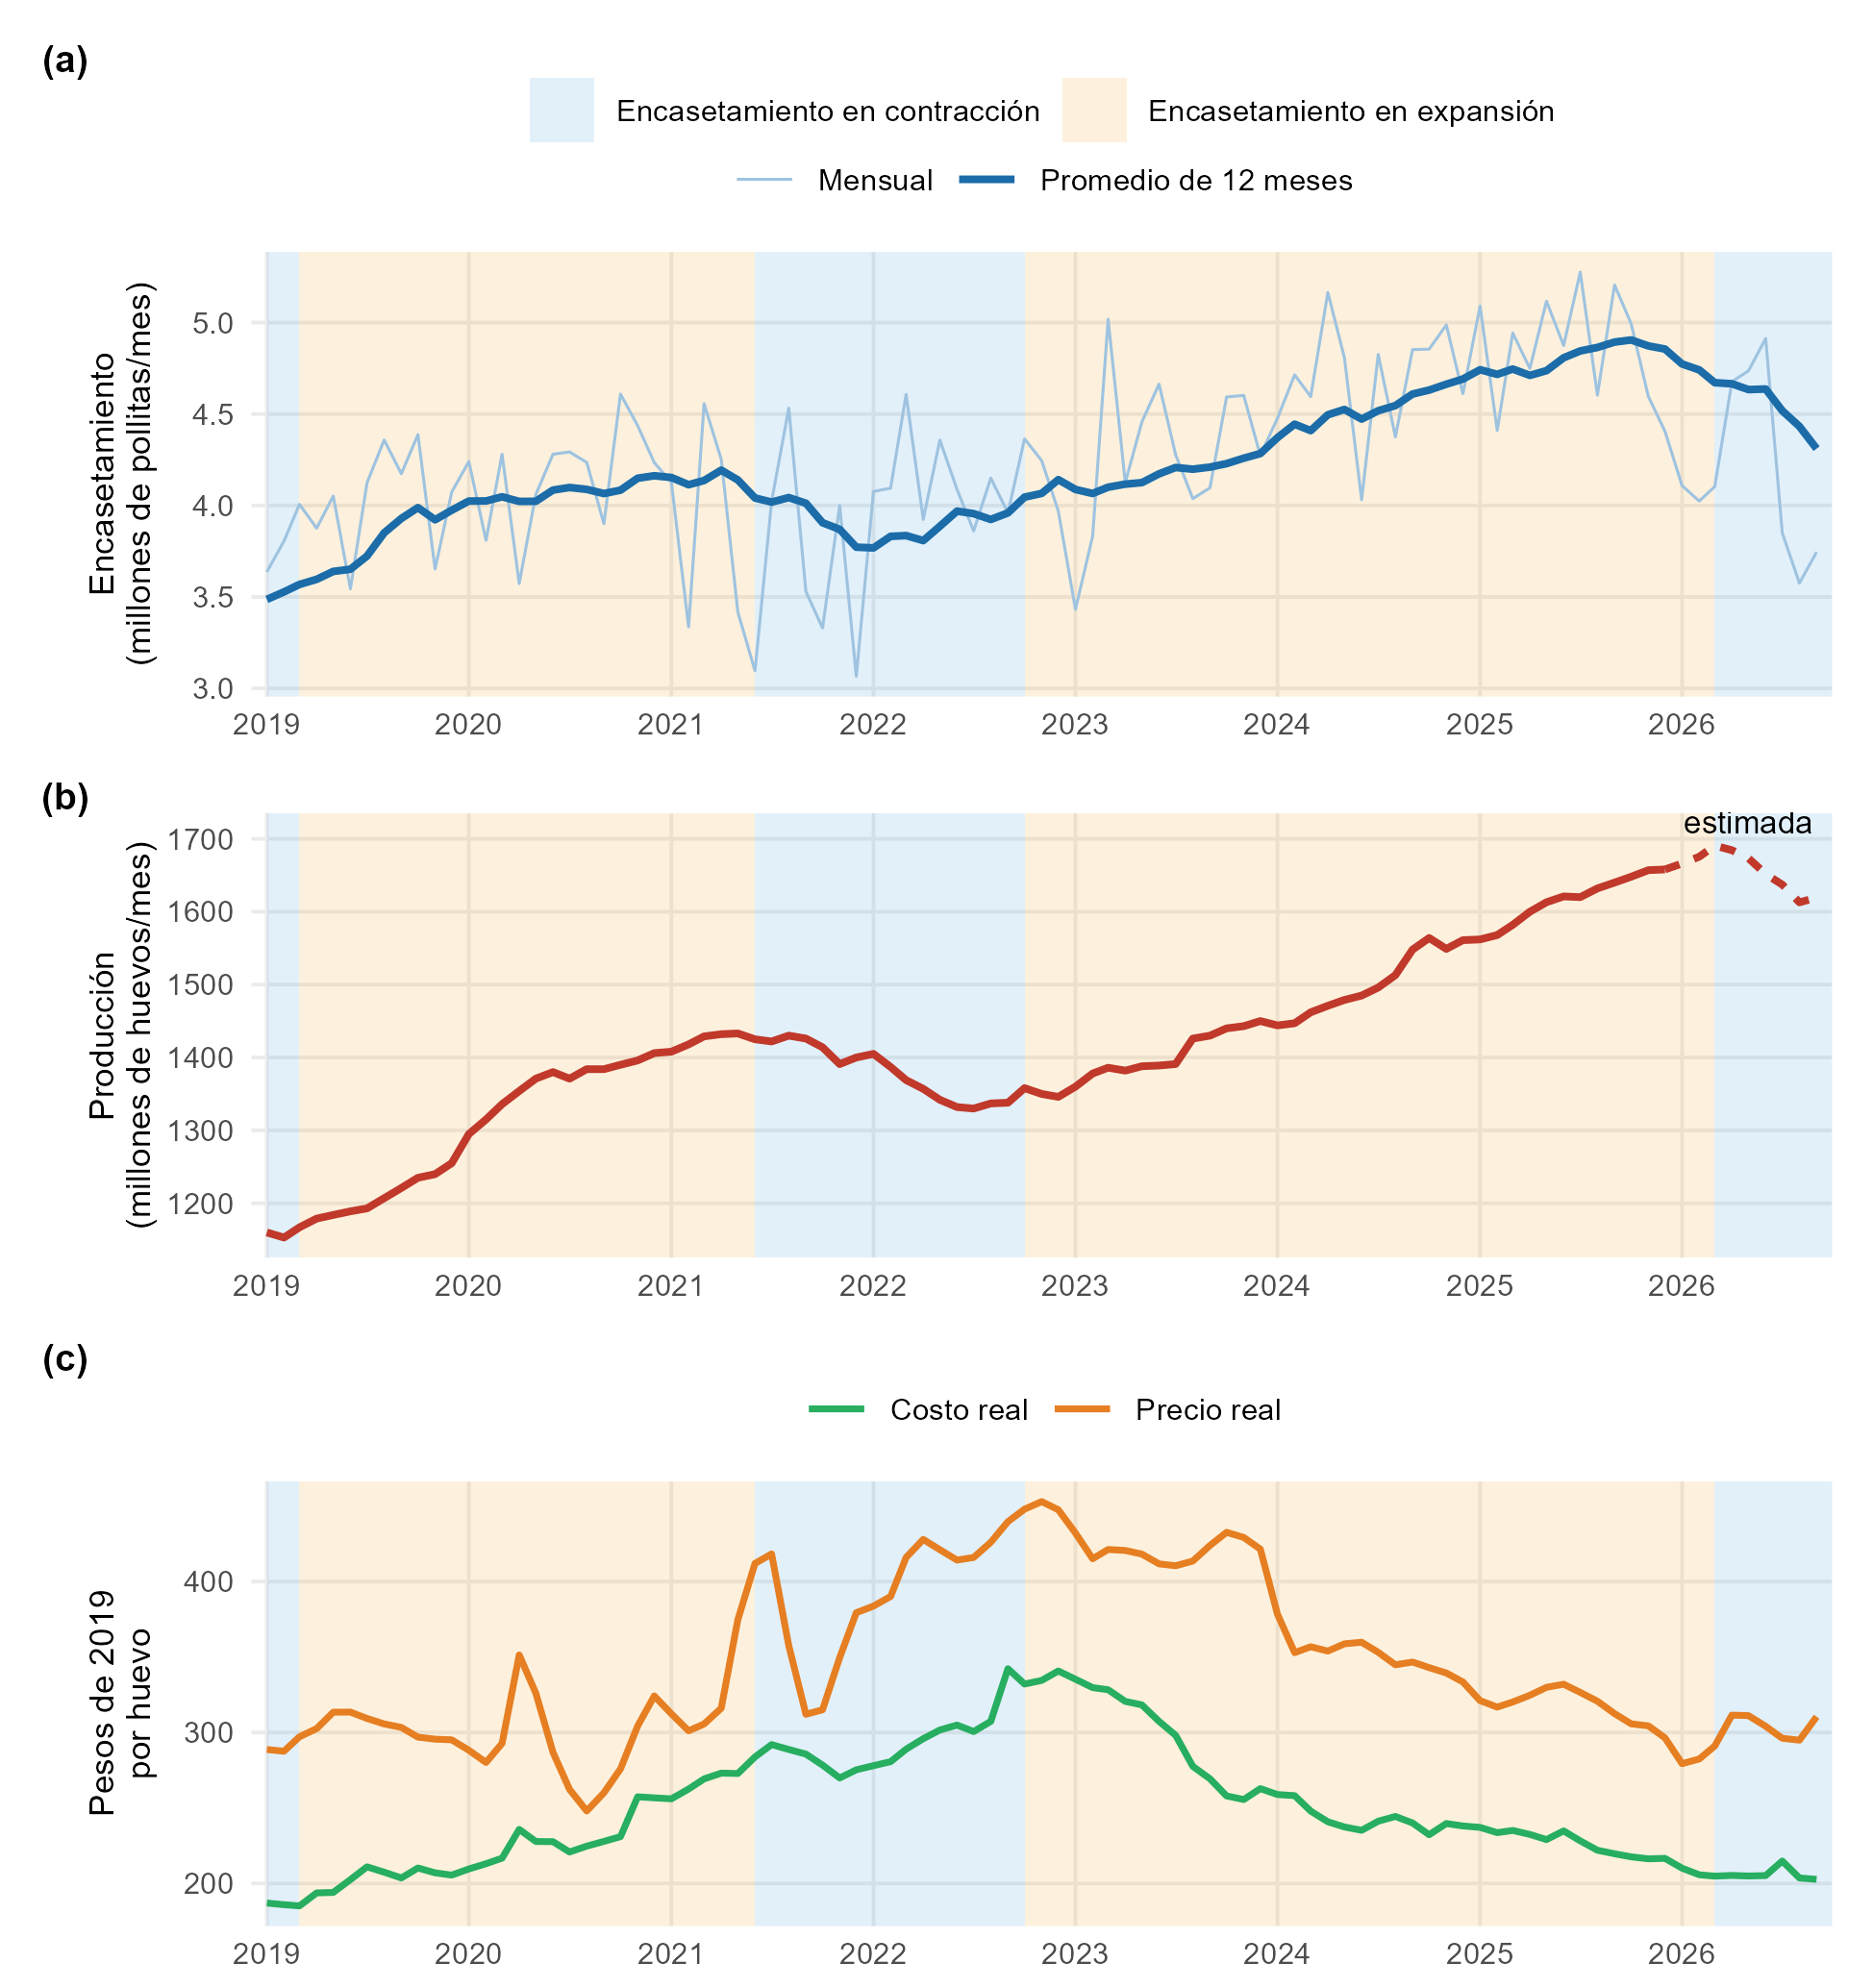
\includegraphics[width=\textwidth]{fig_series_temporales}
\caption{Encasetamiento, producción, precio y costo del huevo en Colombia, 2019--2026. (a) Encasetamiento mensual de pollitas de postura y su promedio de 12 meses; (b) producción mensual de huevo; (c) precio mayorista real del huevo rojo AA y costo real de producción sin amortización del ave, en pesos de 2019. El sombreado sigue el signo de la variación anual del encasetamiento (suma de 12 meses); la línea discontinua es la producción estimada. Fuente: elaboración propia con base en \citet{Fenavi2026Estadisticas,Fenavi2026Costos}, \citet{DANE2026SIPSA} y \citet{DANE2026IPC}.}
\label{fig:series}
\end{figure}

\subsubsection{Las cinco preguntas del problema}

%% Tabla larga: xltabular la parte entre páginas si no cabe en una.
\begingroup\small
\begin{xltabular}{\textwidth}{@{}P{2.2cm}L@{}}
\caption{Formulación del problema del ciclo del huevo en Colombia.}
\label{tab:preguntas}\\
\toprule
Pregunta & Respuesta \\
\midrule
\endfirsthead
\multicolumn{2}{@{}l}{\footnotesize\itshape Tabla~\ref{tab:preguntas} (continuación)}\\
\toprule
Pregunta & Respuesta \\
\midrule
\endhead
\midrule
\multicolumn{2}{r@{}}{\footnotesize\itshape Continúa en la página siguiente}\\
\endfoot
\bottomrule
\multicolumn{2}{@{}p{\textwidth}@{}}{\footnotesize Fuente: elaboración propia.}\\
\endlastfoot
¿Qué? & Una oscilación recurrente de la oferta y del precio del huevo. Cuando el margen es alto, los productores encasetan más pollitas; unas 20 semanas después esas aves entran en postura, la producción crece más que el consumo y el precio cae; con el margen deprimido, el encasetamiento se recorta y se prepara una nueva escasez. La raíz está en la regla de decisión: se encaseta según el precio y el margen corrientes, sin descontar por completo las aves que ya están en levante. \\
\addlinespace
¿Cuánto? & \textit{Encasetamiento:} pasó de 45,3 millones de aves en 2021 a 58,3 millones en 2025 (+28,7~\%) y cayó 14,8~\% entre enero y septiembre de 2026 frente al mismo periodo de 2025, de 44,27 a 37,73 millones \citep{Fenavi2026Estadisticas}.\par
\textit{Producción:} pasó de 16.251 millones de huevos en 2022 a 19.401 millones en 2025 (+19,4~\%) \citep{Fenavi2026Estadisticas}.\par
\textit{Precio:} el precio mayorista real del huevo rojo AA subió 22,4~\% en 2022 y bajó 16,4~\% en 2024 y 9,7~\% en 2025, en pesos de 2019 \citep{DANE2026IPC,DANE2026SIPSA}.\par
\textit{Costo:} el costo por huevo sin amortización del ave subió de 208 pesos en diciembre de 2019 a 421,8 pesos en marzo de 2023 (+103~\%, en pesos corrientes) y bajó a 318 pesos en promedio en 2026 \citep{Fenavi2026Costos}.\par
\textit{Margen:} la razón entre el precio mayorista y el costo osciló entre 1,09 (septiembre de 2021) y 1,68 (noviembre de 2023); con el precio que recibe el productor, que es menor que el mayorista, Fenavi registró márgenes brutos aparentes negativos desde octubre de 2025 \citep{Fenavi2026Fenaviquin440}.\par
\textit{Capacidad:} la capacidad de postura instalada creció de 69,6 a 80,4 millones de aves entre los censos de 2019 y 2025 (+15,6~\%), mientras la ocupación bajó de 89,4~\% (2022) a 83,7~\% (2025), con unos 13,1 millones de cupos sin usar \citep{ICA2025Censo}.\par
\textit{Productores:} en 2024 y 2025, 1.614 productores sin registro previo encasetaron 6,83 millones de pollitas \citep{Fenavi2026Fenaviquin440}. \\
\addlinespace
¿Cuándo? & En el periodo 2019--2026, que el modelo extiende hasta 2030. La caída del encasetamiento de 2021 antecedió a la menor producción de 2022 y a una fase de precios altos: la variación anual del índice de precios al consumidor (IPC) del huevo llegó a 31,97~\% en marzo de 2022 \citep{DANE2026IPC}. La expansión de 2022 a 2025 desembocó en la sobreoferta y la caída del precio de 2024 y 2025, y después llegaron los márgenes negativos, las protestas de enero de 2026 y el recorte del encasetamiento. Un análisis bancario anticipa por ello menor oferta y una probable recuperación del precio en 2027 \citep{Portafolio2026}; es una proyección, no un dato observado. \\
\addlinespace
¿Dónde? & En el mercado colombiano del huevo, que es nacional: el precio se forma en las centrales mayoristas que sigue el SIPSA \citep{DANE2026SIPSA} y la producción se reparte en 2.558 predios de postura registrados en el censo del ICA de 2025 \citep{ICA2025Censo}. El estudio pone el énfasis en el Valle del Cauca, uno de los principales departamentos productores: solo en Santiago de Cali, 23 productores nuevos encasetaron 175.381 pollitas en 2024 y 2025 \citep{Fenavi2026Fenaviquin440}. \\
\addlinespace
¿A quién afecta? & A los avicultores, sobre todo a los pequeños y a los que entraron durante la bonanza, que absorben las pérdidas en la fase de sobreoferta y que en 2026 protestaron para pedir la regulación del encasetamiento y un fondo de estabilización de precios \citep{Villamizar2026}.\par
A los hogares, para quienes el huevo es una de las proteínas animales de menor costo y que pagan precios altos en la fase de escasez.\par
A los proveedores de genética, alimento balanceado y servicios veterinarios, cuya demanda sigue el ritmo del encasetamiento, y a los intermediarios y comercializadores.\par
Al gremio y a las autoridades del sector (Fenavi y el Fondo Nacional Avícola, el ICA y el Ministerio de Agricultura), que reciben la presión para intervenir el mercado. \\
\end{xltabular}
\endgroup

\subsubsection{Señales del problema y causas derivadas}

Las señales de resultados son lo que perciben productores y hogares (el precio y el margen); las de procesos, lo que se observa en la operación del sector (aves que entran, producción y capacidad); y las causas derivadas, las condiciones que conectan unas con otras (Tabla~\ref{tab:senales}).

\begin{table}[!htbp]
\centering
\caption{Señales del problema y causas derivadas.}
\label{tab:senales}
\footnotesize
\setlength{\tabcolsep}{4pt}
\begin{tabularx}{\textwidth}{@{}P{3.6cm}P{4.2cm}L@{}}
\toprule
Señales de resultados & Señales de procesos & Causas derivadas \\
\midrule
Precio real con alzas fuertes en 2021 y 2022 y caídas en 2024 y 2025.\par\smallskip
Razón precio/costo que oscila entre 1,09 y 1,68.\par\smallskip
Márgenes negativos desde octubre de 2025 y protestas de productores en enero de 2026.
&
Encasetamiento que alterna expansión (2019 y 2022--2025) y contracción (2021 y 2026).\par\smallskip
Producción que repite el encasetamiento de 13 a 15 meses después.\par\smallskip
Capacidad instalada que crece más rápido que las aves alojadas.\par\smallskip
Entrada de 1.614 productores nuevos en 2024 y 2025.
&
1. Se encaseta según el precio y el margen corrientes, que el productor percibe con rezago.\par\smallskip
2. El productor ve sus aves en levante, pero no las del resto del sector, que se publican como cifra mensual agregada.\par\smallskip
3. Las demoras biológicas son largas: 20 semanas de levante y unas 60 de postura \citep{Fenavi2026Fenaviquin440}.\par\smallskip
4. En las bonanzas entran productores y se amplían galpones; esa capacidad casi no sale cuando el precio cae.\par\smallskip
5. La demanda responde poco al precio (elasticidad de $-$0,46): una sobreoferta pequeña mueve mucho el precio \citep{TorresCastro2016}.\par\smallskip
6. Cerca del 70~\% del costo es alimento hecho con maíz y soya importados \citep{Fenavi2026Fenaviquin456,USDAFAS2025}. \\
\bottomrule
\end{tabularx}

\smallskip
{\footnotesize\raggedright Las magnitudes y sus fuentes están en la Tabla~\ref{tab:preguntas}. Fuente: elaboración propia con el análisis funcional de \citet{RubianoVillarreal}.\par}
\end{table}

\subsubsection{Definición del problema}

\noindent Con las señales y las causas anteriores, el problema se define así:

\medskip
\noindent \textit{Las decisiones de encasetamiento, basadas en el precio y el margen corrientes y en una visión parcial de las aves que ya están en levante, se combinan con una demora biológica de unas 20 semanas, una vida productiva de unas 60 semanas y la entrada de productores atraídos por la rentabilidad. El resultado son oscilaciones de la producción y del precio del huevo en Colombia que llevan a los avicultores a pérdidas en las fases de sobreoferta y a los hogares a pagar precios altos en las fases de escasez.}

%% -------------------------------------------------------------------
\subsection{Descripción del sistema}
\label{sec3.3}

El sistema es la cadena del huevo de mesa en Colombia, desde la entrada de pollitas de un día a las granjas hasta el consumo de los hogares. La Tabla~\ref{tab:sipoc} lo resume en un diagrama SIPOC y la Figura~\ref{fig:flujos} muestra sus flujos de materiales, información y decisiones.

\begin{table}[!htbp]
\centering
\caption{Diagrama SIPOC de la cadena del huevo.}
\label{tab:sipoc}
\footnotesize
\setlength{\tabcolsep}{4pt}
\begin{tabularx}{\textwidth}{@{}LLLLL@{}}
\toprule
Proveedores & Entradas & Proceso & Salidas & Clientes \\
\midrule
Casas genéticas e incubadoras\newline
Fábricas de alimento balanceado\newline
Importadores de maíz y torta de soya\newline
Laboratorios veterinarios\newline
Constructores de galpones y bancos
&
Pollitas de un día\newline
Alimento balanceado\newline
Vacunas y medicamentos\newline
Galpones y equipos\newline
Mano de obra y capital
&
Encasetamiento\newline
Levante y prepostura ($\approx$\,20 semanas)\newline
Postura ($\approx$\,60 semanas)\newline
Recolección, clasificación y empaque\newline
Distribución\newline
Descarte o replume
&
Huevo por categorías (B, A, AA, AAA y jumbo)\newline
Gallina de descarte\newline
Gallinaza
&
Hogares\newline
Centrales mayoristas\newline
Tiendas y supermercados\newline
Industria de alimentos\newline
Exportación (marginal) \\
\bottomrule
\end{tabularx}

\smallskip
{\footnotesize\raggedright Fuente: elaboración propia con base en \citet{Fenavi2026Fenaviquin440}.\par}
\end{table}

\subsubsection{Proceso productivo}

El proceso empieza en las casas genéticas y las incubadoras, que venden pollitas de un día. En 2025 el potencial genético de pollitas de postura fue de 69,18 millones, frente a un encasetamiento de 58,3 millones \citep{Fenavi2026Fenaviquin456}; la oferta de pollitas no limita el sistema y la cantidad que entra la decide el productor.

El encasetamiento es el ingreso de las pollitas a la granja. Las aves pasan por el levante y la prepostura, unas 20 semanas en las que se alimentan, se vacunan y alcanzan la madurez. En el censo de 2025 el ICA registró 214 predios especializados en levante, con 8,0 millones de aves alojadas \citep{ICA2025Censo}, aunque buena parte del levante se hace en las mismas granjas de postura. Entre las semanas 18 y 20 las aves empiezan a poner huevos pequeños y siguen en postura hasta cerca de la semana 80; en ese ciclo una gallina produce unos 350 huevos y la mortalidad ronda el 12~\% \citep{Fenavi2026Fenaviquin440}. Según el mismo censo, la capacidad de postura instalada era de 80,4 millones de aves en 2.558 predios, con 67,3 millones de aves alojadas \citep{ICA2025Censo}.

Al final de la postura, el productor decide si descarta la gallina, que se vende como gallina de descarte, o si la somete a una muda forzada para obtener un segundo ciclo de postura, más corto. La vida productiva depende, por tanto, del precio (sección~\ref{sec2.5}). El huevo se recolecta, se clasifica por peso en las categorías B, A, AA, AAA y jumbo, y se empaca. Después se distribuye a las centrales mayoristas, a las tiendas de barrio y los supermercados, a la industria de alimentos y, en menor medida, a la exportación, que entre enero y noviembre de 2025 sumó 36,9 millones de huevos, cerca del 0,2~\% de la producción del año \citep{Fenavi2026Rueda}. La gallinaza se aprovecha como abono.

\subsubsection{Insumos, costos y formación del precio}

%% El borrador decía "en junio de 2026 representó el 69,7 % del costo [35]".
%% El texto de Fenaviquín 456 menciona 72 % para el huevo: confirmar la página
%% y la definición antes de dar una cifra exacta.
El principal insumo es el alimento balanceado, que representa cerca del 70~\% del costo por huevo \citep{Fenavi2026Fenaviquin456}. La fórmula se basa en maíz amarillo y torta de soya, en su mayoría importados \citep{USDAFAS2025}. Por eso el costo por huevo depende del precio internacional de esas materias primas y de la tasa de cambio: se duplicó entre 2019 y 2023 y, en pesos de 2019, bajó cerca de 40~\% entre su máximo de septiembre de 2022 y 2026 (Figura~\ref{fig:series}c) \citep{Fenavi2026Costos}. Los demás costos son la mano de obra, que sigue al salario mínimo, la sanidad, la energía y la amortización de las aves y de los galpones.

El precio se forma en el mercado mayorista según la relación entre la oferta y la demanda. El SIPSA lo publica a diario y por semana para varias categorías de huevo en las principales centrales del país \citep{DANE2026SIPSA}. El precio que recibe el productor en la granja es menor que el mayorista: Fenavi advierte que el precio del SIPSA incluye el margen de comercialización y de los intermediarios y no corresponde al precio del productor \citep{Fenavi2024Fenaviquin394}. Por esa razón el precio mayorista sirve como señal del mercado, pero no como medida directa del ingreso del productor, y el modelo distingue los dos. La demanda responde poco al precio: con datos mensuales de 1999 a 2015 se estimó una elasticidad precio de $-$0,462 \citep{TorresCastro2016}, de modo que una sobreoferta pequeña produce una caída grande del precio.

\subsubsection{Flujos de información y decisiones}

La Figura~\ref{fig:flujos} integra el proceso físico con las decisiones y con la información que las alimenta. El productor toma tres decisiones: cuántas pollitas encasetar, si amplía sus galpones y cuándo descartar o someter a muda a las gallinas. Las tres responden al margen percibido, que el productor forma al comparar el precio que observa, con algún rezago, con su costo unitario. La decisión de encasetar depende además de las gallinas que el productor quiere tener para atender la demanda esperada y de las que ya tiene, y la toman tanto los productores establecidos como los que entran al negocio atraídos por la rentabilidad.

\begin{figure}[!htbp]
\centering
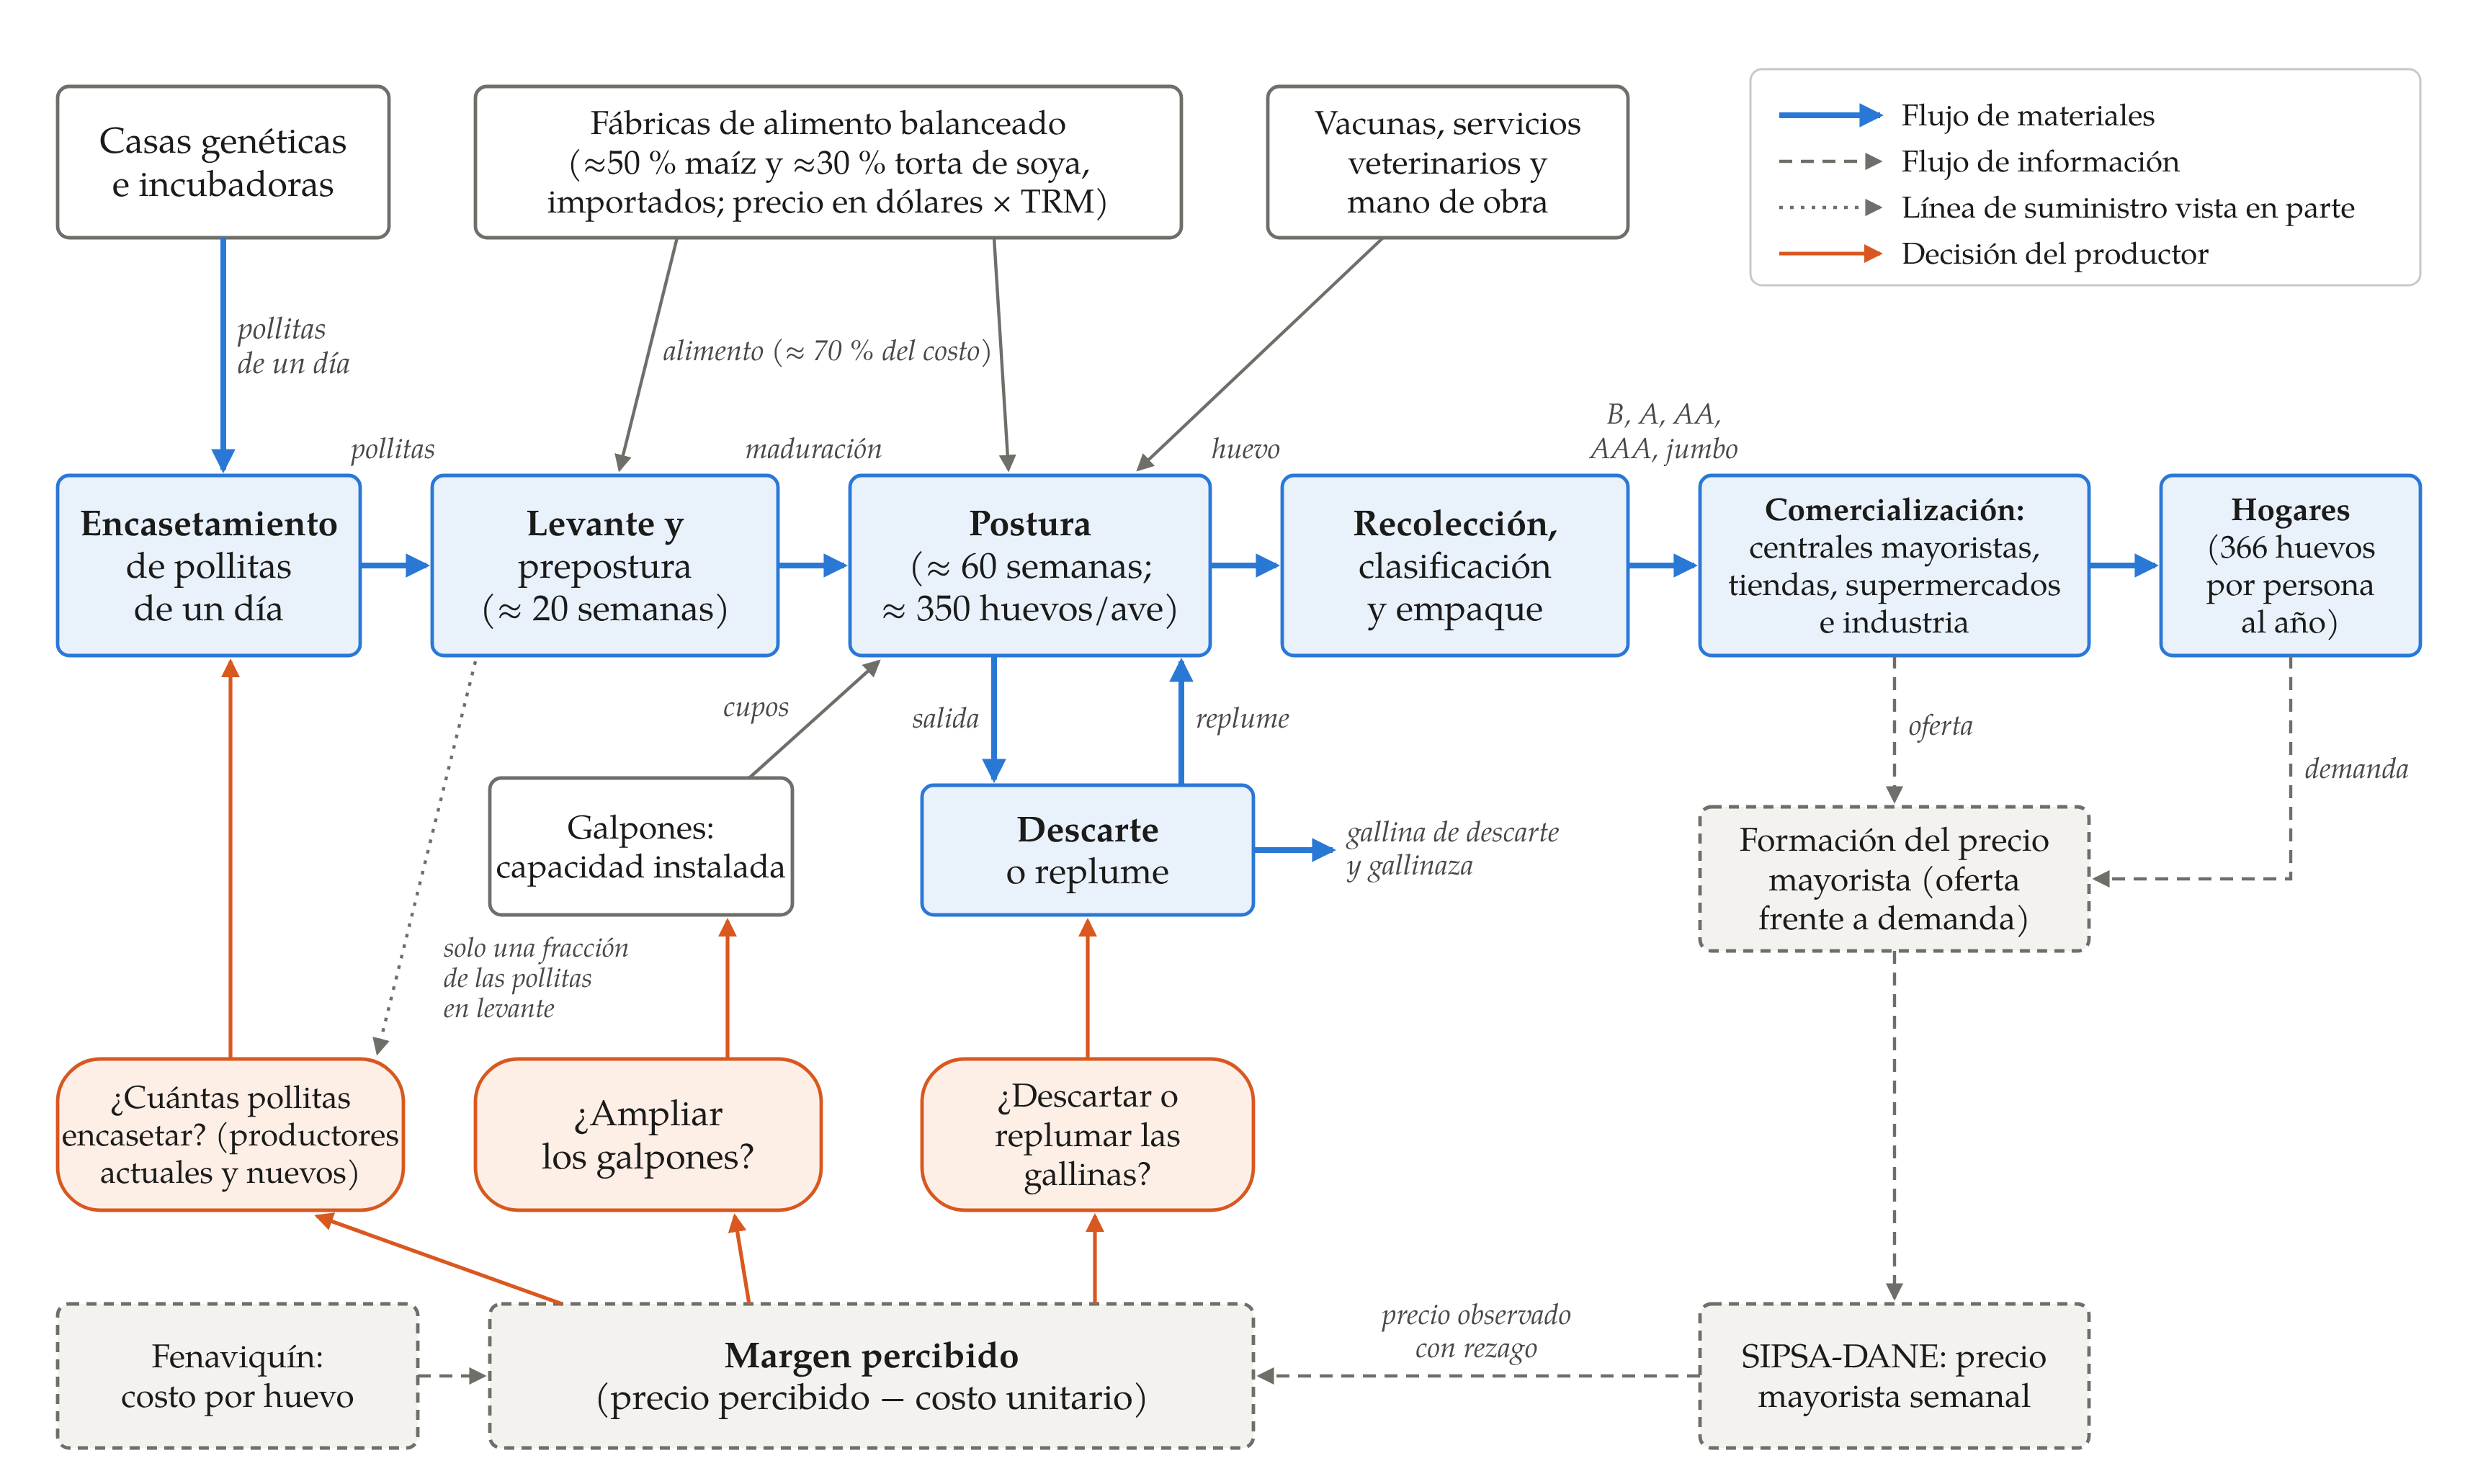
\includegraphics[width=\textwidth]{fig_flujos_cadena_huevo}
\caption{Flujos de materiales, información y decisiones en la cadena del huevo. Las flechas azules son flujos de materiales; las grises discontinuas, flujos de información; la punteada, la información incompleta sobre las pollitas en levante; y las naranjas, las decisiones del productor. Fuente: elaboración propia con base en \citet{Hollingsworth1995} y \citet{Fenavi2026Fenaviquin440}.}
\label{fig:flujos}
\end{figure}

El sistema tiene tres demoras que separan cada decisión de su efecto: la percepción del precio, que se observa en el mercado mayorista y llega al productor con rezago; el levante, de unas 20 semanas entre el encasetamiento y la primera postura; y la vida productiva, de unas 60 semanas, durante las cuales cada lote sigue aportando huevo aunque el precio haya caído. A ellas se suma una brecha de información, la línea punteada de la Figura~\ref{fig:flujos}: el productor conoce sus propias aves, pero el encasetamiento del resto del sector solo se publica como cifra mensual agregada, y las personas tienden a subestimar lo que ya está en camino (sección~\ref{sec2.3}).

%% -------------------------------------------------------------------
\subsection{Datos y evidencia de los retardos}
\label{sec3.4}

Para el estudio se construyó una base de datos semanal, mensual y anual con las series de la Tabla~\ref{tab:datos}, con datos hasta septiembre de 2026. Las series se llevaron a frecuencia semanal y mensual; los precios y los costos se deflactaron con el IPC y se expresan en pesos de 2019. La producción de enero a septiembre de 2026, aún sin publicar, se estimó con el encasetamiento de los 5 a 18 meses anteriores, con un error medio de 0,58~\% frente a los datos de Fenavi de 2019 a 2025. Como Fenavi también calcula la producción a partir del encasetamiento, el rezago entre las dos series ilustra la demora biológica, pero no es una prueba independiente de ella. El margen se aproxima con la razón entre el precio mayorista y el costo de producción sin amortización del ave. Esa razón mide la holgura del margen y no la utilidad del productor, porque el precio mayorista incluye el margen de los intermediarios y el costo deja por fuera la amortización de la pollita.

\begin{table}[!htbp]
\centering
\caption{Datos utilizados.}
\label{tab:datos}
\footnotesize
\setlength{\tabcolsep}{4pt}
\begin{tabularx}{\textwidth}{@{}P{3.0cm}P{2.1cm}P{1.5cm}P{2.1cm}L@{}}
\toprule
Variable & Unidad & Frecuencia & Periodo & Fuente \\
\midrule
Encasetamiento de pollitas de postura & pollitas/mes & Mensual & ene-2017 a sep-2026 & \citet{Fenavi2026Estadisticas} \\
Producción de huevo & millones de huevos/mes & Mensual & ene-2017 a dic-2025 (2026 estimada) & \citet{Fenavi2026Fenaviquin440}; 2026: estimación propia \\
Precio mayorista del huevo rojo AA & pesos/unidad & Mensual & ene-2017 a sep-2026 & \citet{DANE2026SIPSA}, promedio de 19 mercados \\
Costo de producción por huevo & pesos/unidad & Mensual & ene-2019 a sep-2026 & \citet{Fenavi2026Costos}, sin amortización del ave \\
Índice de precios al consumidor & dic-2018 = 100 & Mensual & ene-2017 a sep-2026 & \citet{DANE2026IPC} \\
Precio del maíz amarillo & US\$/tonelada & Mensual & ene-2017 a sep-2026 & \citet{WorldBank2026PinkSheet} \\
Precio de la torta de soya & US\$/tonelada & Mensual & ene-2017 a sep-2026 & \citet{WorldBank2026PinkSheet} \\
Tasa representativa del mercado (TRM) & pesos/US\$ & Diaria & ene-2017 a sep-2026 & \citet{BanRep2026} \\
Salario mínimo & pesos/mes & Anual & 2017 a 2026 & \citet{BanRep2026} \\
Población & personas & Anual (30 de junio) & 2018 a 2028 & \citet{DANE2025Poblacion} \\
Capacidad instalada de postura & aves & Anual & 2019 a 2025 & \citet{ICA2025Censo} \\
\bottomrule
\end{tabularx}

\smallskip
{\footnotesize\raggedright Todas las series se llevan a frecuencia semanal y mensual en la base de datos del modelo. Fuente: elaboración propia.\par}
\end{table}

La Tabla~\ref{tab:fases} resume el ciclo año por año. Los años de margen alto (2019, 2023 y 2024) preceden la expansión del encasetamiento y de la capacidad instalada, y uno o dos años después crece la producción y cae el precio real. Los márgenes estrechos de 2020 y 2021 precedieron la contracción del encasetamiento de 2021, la menor producción de 2022 y las alzas del precio.

\begin{table}[!htbp]
\centering
\caption{Fases del ciclo del huevo en Colombia, 2019--2026.}
\label{tab:fases}
\footnotesize
\setlength{\tabcolsep}{3pt}
\begin{tabular}{@{}lC{1.7cm}C{1.8cm}C{1.8cm}C{1.8cm}C{1.8cm}C{1.8cm}@{}}
\toprule
 & Nivel & \multicolumn{5}{c}{Variación anual (\%)} \\
\cmidrule(l){2-2}\cmidrule(l){3-7}
Año & Razón precio/costo & Encaseta-\newline miento & Capacidad de postura (ICA) & Producción & Consumo por habitante & Precio real \\
\midrule
2019 & 1,51 & +14,8 & --- & $-$1,5 & $-$3,6 & +8,9 \\
2020 & 1,27 & +4,7 & +4,2 & +13,9 & +11,4 & $-$3,0 \\
2021 & 1,25 & $-$9,4 & $-$2,1 & +3,9 & +2,5 & +18,7 \\
2022 & 1,37 & +9,8 & +3,5 & $-$4,6 & $-$5,5 & +22,4 \\
2023 & 1,43 & +3,4 & +1,9 & +3,8 & +2,8 & $-$0,6 \\
2024 & 1,45 & +9,5 & $-$2,4 & +6,9 & +5,8 & $-$16,4 \\
2025 & 1,40 & +3,5 & +10,2 & +7,7 & +6,8 & $-$9,7 \\
\midrule
2026\textsuperscript{a} & 1,44 & $-$14,8 & --- & +3,3 & +2,6 & $-$7,7 \\
\bottomrule
\end{tabular}

\smallskip
{\footnotesize\raggedright Razón = precio mayorista / costo sin amortización del ave (promedio 2019--2025: 1,39). \textsuperscript{a}~Enero a septiembre de 2026 frente al mismo periodo de 2025, con producción estimada. Fuente: elaboración propia con base en \citet{Fenavi2026Estadisticas}, \citet{DANE2026SIPSA}, \citet{DANE2025Poblacion} y \citet{ICA2025Censo}.\par}
\end{table}

El ciclo se cierra con cuatro eslabones, cada uno con su retardo; la Tabla~\ref{tab:eslabones} reúne los retardos y las correlaciones. En el primero, del encasetamiento a la producción, cada pico o valle del encasetamiento reaparece en la producción entre 13 y 15 meses después (Figura~\ref{fig:rezago}), y con datos semanales la correlación es positiva entre las semanas 20 y 80, que son las de la postura (Figura~\ref{fig:correlacion}a).

\begin{figure}[!htbp]
\centering
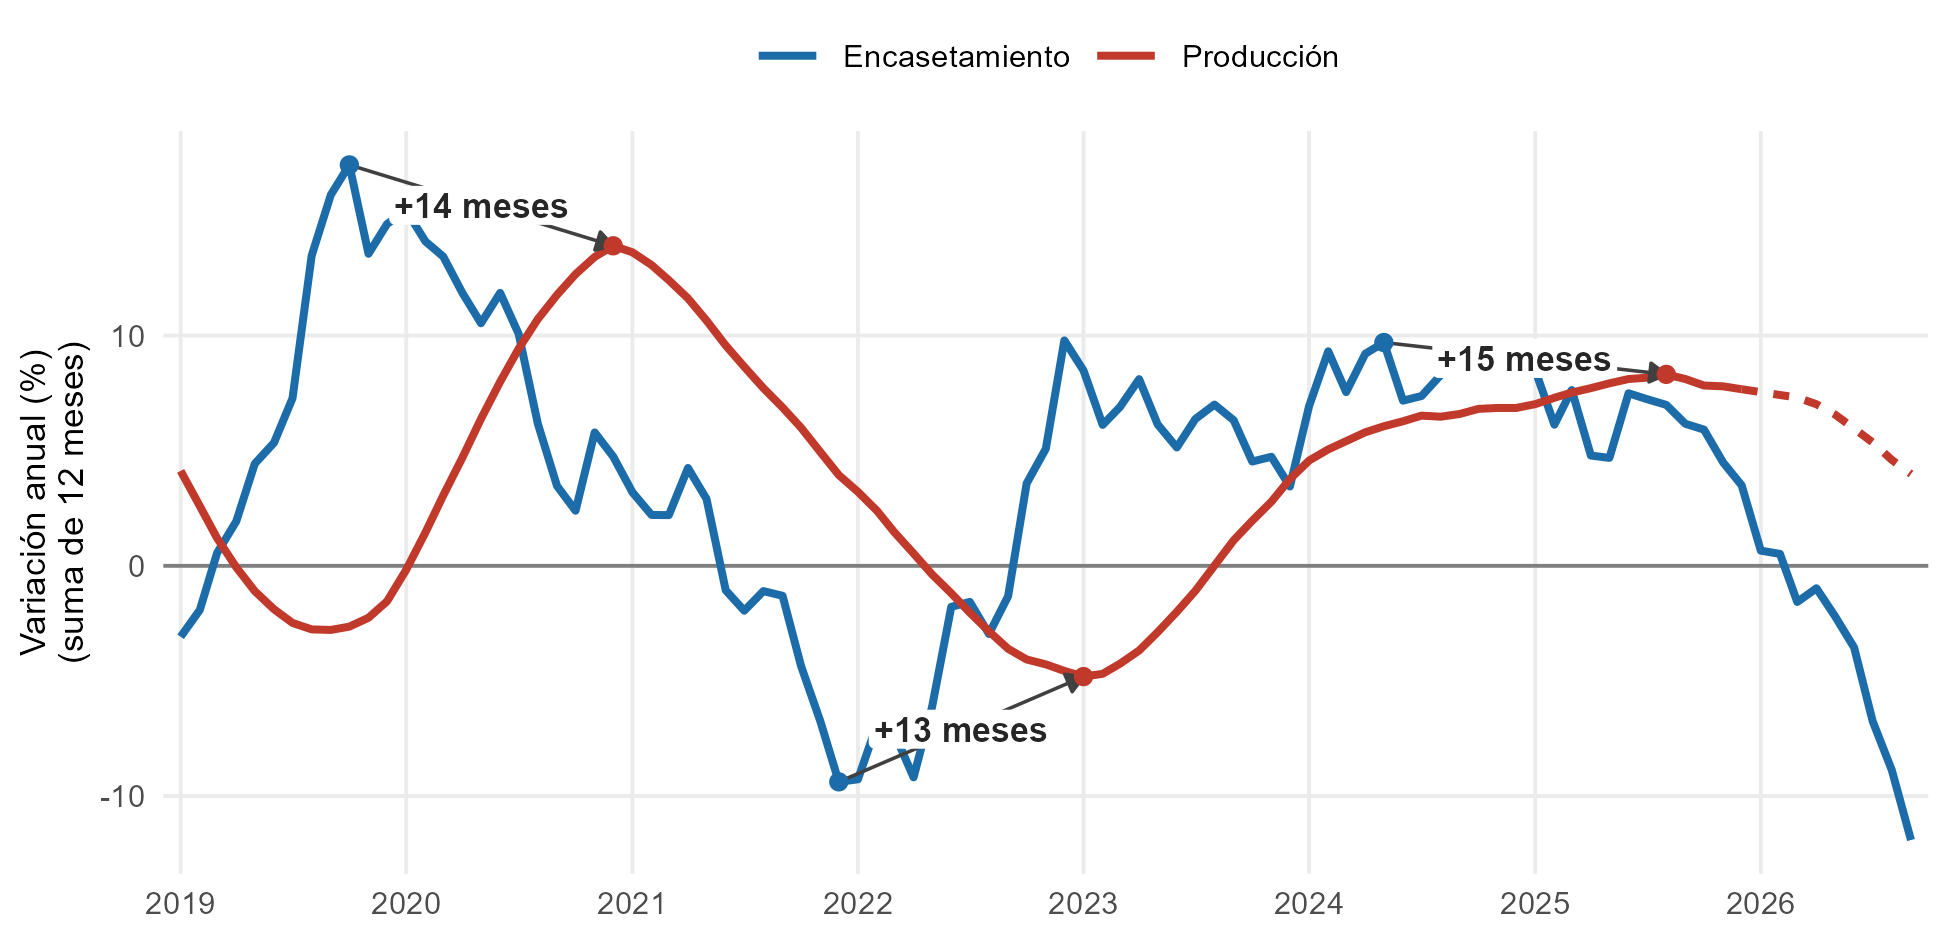
\includegraphics[width=\textwidth]{fig_rezago_encasetamiento_produccion}
\caption{Variación anual del encasetamiento y de la producción de huevo, 2019--2026 (suma de 12 meses frente a los 12 anteriores). Las flechas unen cada pico o valle del encasetamiento (extremo en una ventana de $\pm$12 meses) con el de la producción entre 6 y 18 meses después. Línea discontinua: producción estimada. Fuente: elaboración propia con base en \citet{Fenavi2026Estadisticas}.}
\label{fig:rezago}
\end{figure}

El segundo, de la producción al precio, no tiene rezago apreciable. Para separar la sobreoferta del crecimiento normal del consumo, la Figura~\ref{fig:sobreoferta} compara la producción por habitante y el precio real con sus tendencias: cuando la producción supera la suya, como en 2020 y 2021 o desde finales de 2024, el precio real queda por debajo de la suya, y cuando falta producción, como en 2022 y 2023, sube hasta un 30~\% sobre ella.

\begin{figure}[!htbp]
\centering
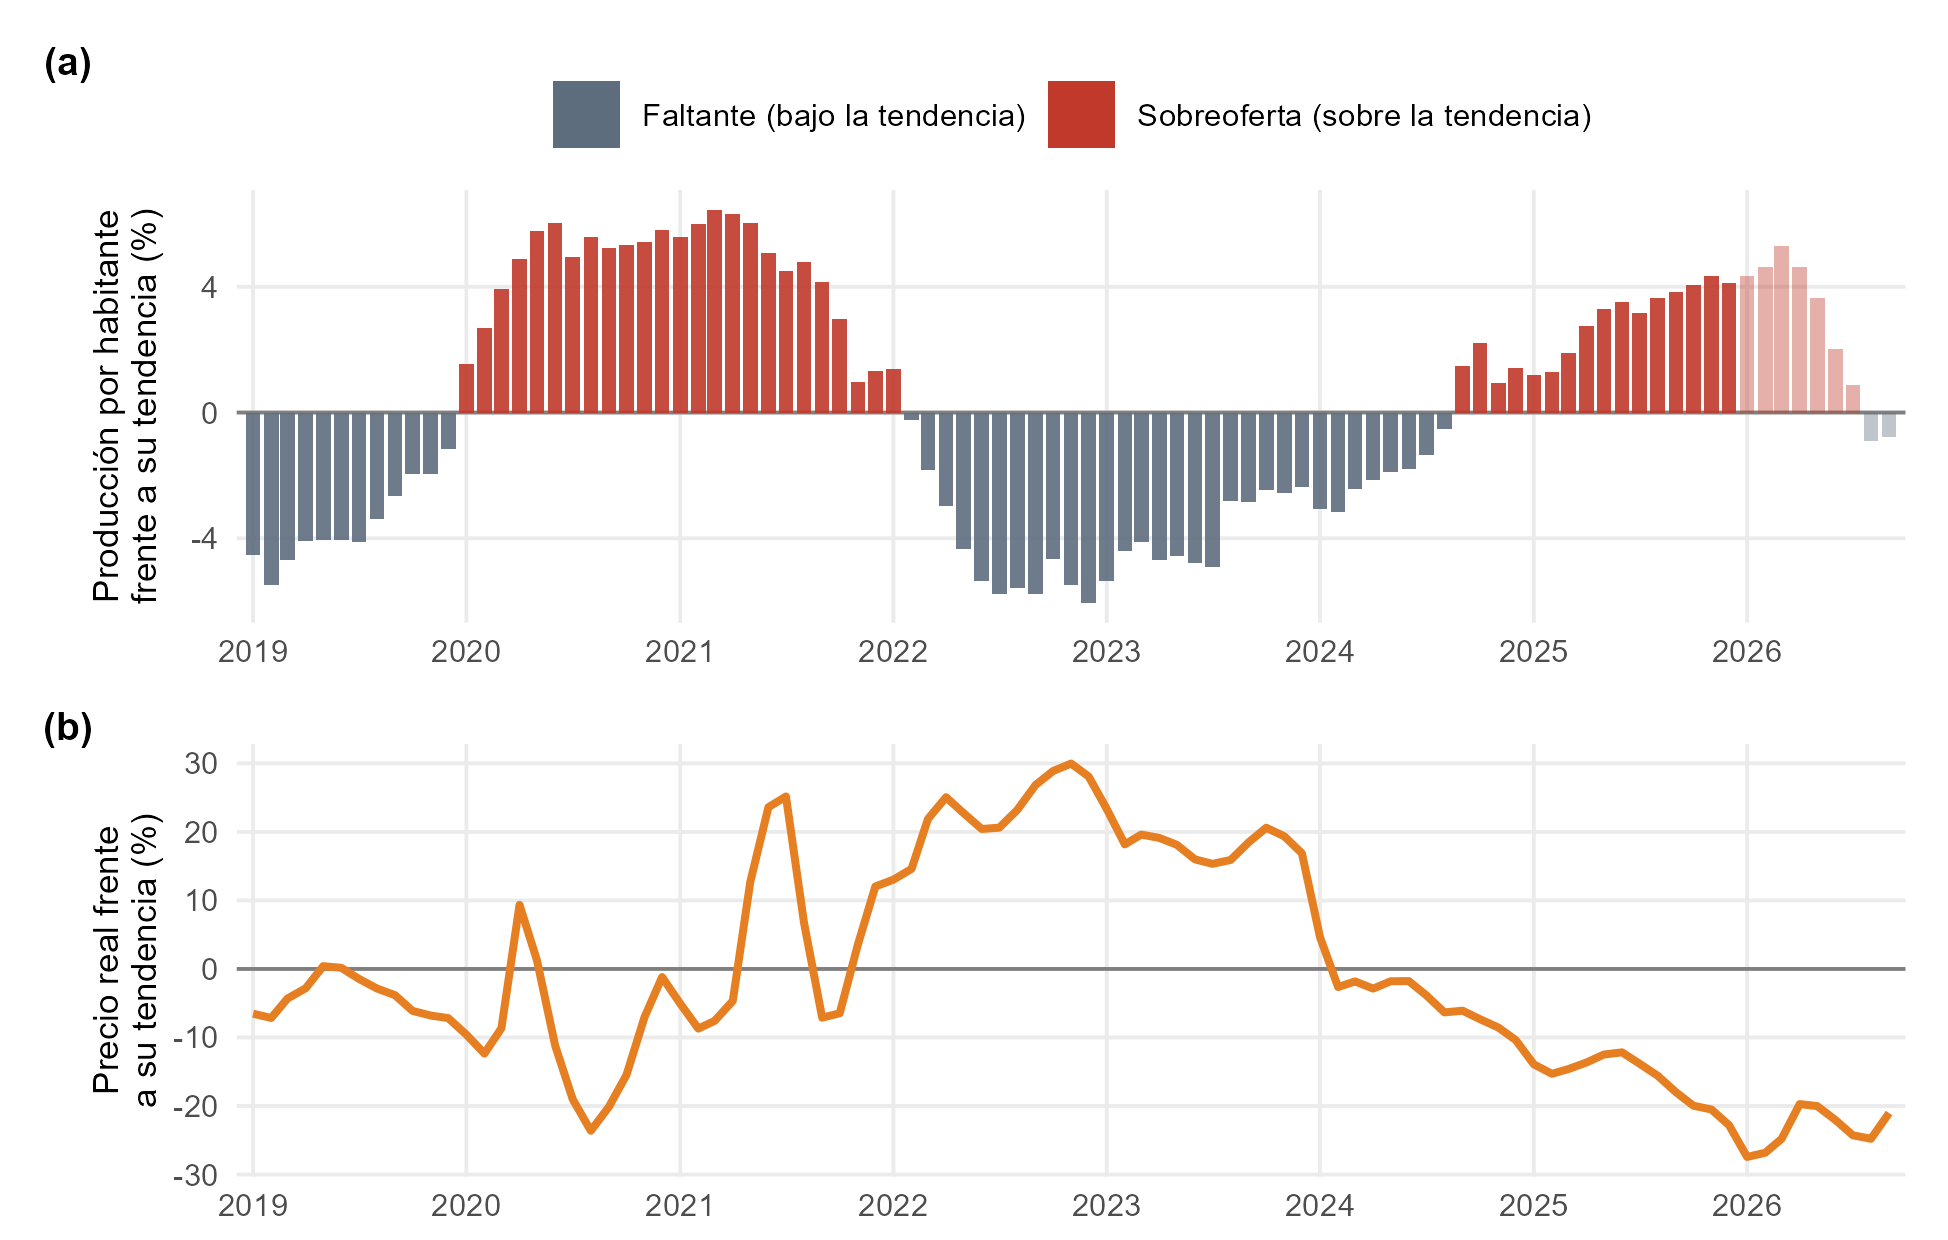
\includegraphics[width=\textwidth]{fig_sobreoferta_precio}
\caption{Sobreoferta de huevo y precio real, 2019--2026. (a) Producción por habitante frente a su tendencia; (b) precio real del huevo frente a su tendencia. Tendencias log-lineales estimadas con datos de julio de 2018 a diciembre de 2025; la de la producción por habitante, de 2,7~\% al año, se toma como el consumo que el mercado absorbe sin cambiar el precio. Barras claras: producción de 2026 estimada. Fuente: elaboración propia con base en \citet{Fenavi2026Estadisticas}, \citet{DANE2026SIPSA} y \citet{DANE2025Poblacion}.}
\label{fig:sobreoferta}
\end{figure}

El tercero, del precio al margen, es inmediato, porque el costo depende de insumos exógenos. El cuarto, del margen a la decisión de encasetar, es el más lento: el margen estrecho de 2020 y 2021 precede la caída del encasetamiento de finales de 2021, el máximo de noviembre de 2023 precede la expansión de 2024 y 2025, y su descenso precede el recorte de 2026 (Figura~\ref{fig:margen}). La correlación entre los dos es positiva entre 7 y 16 meses después (Figura~\ref{fig:correlacion}b).

\begin{figure}[!htbp]
\centering
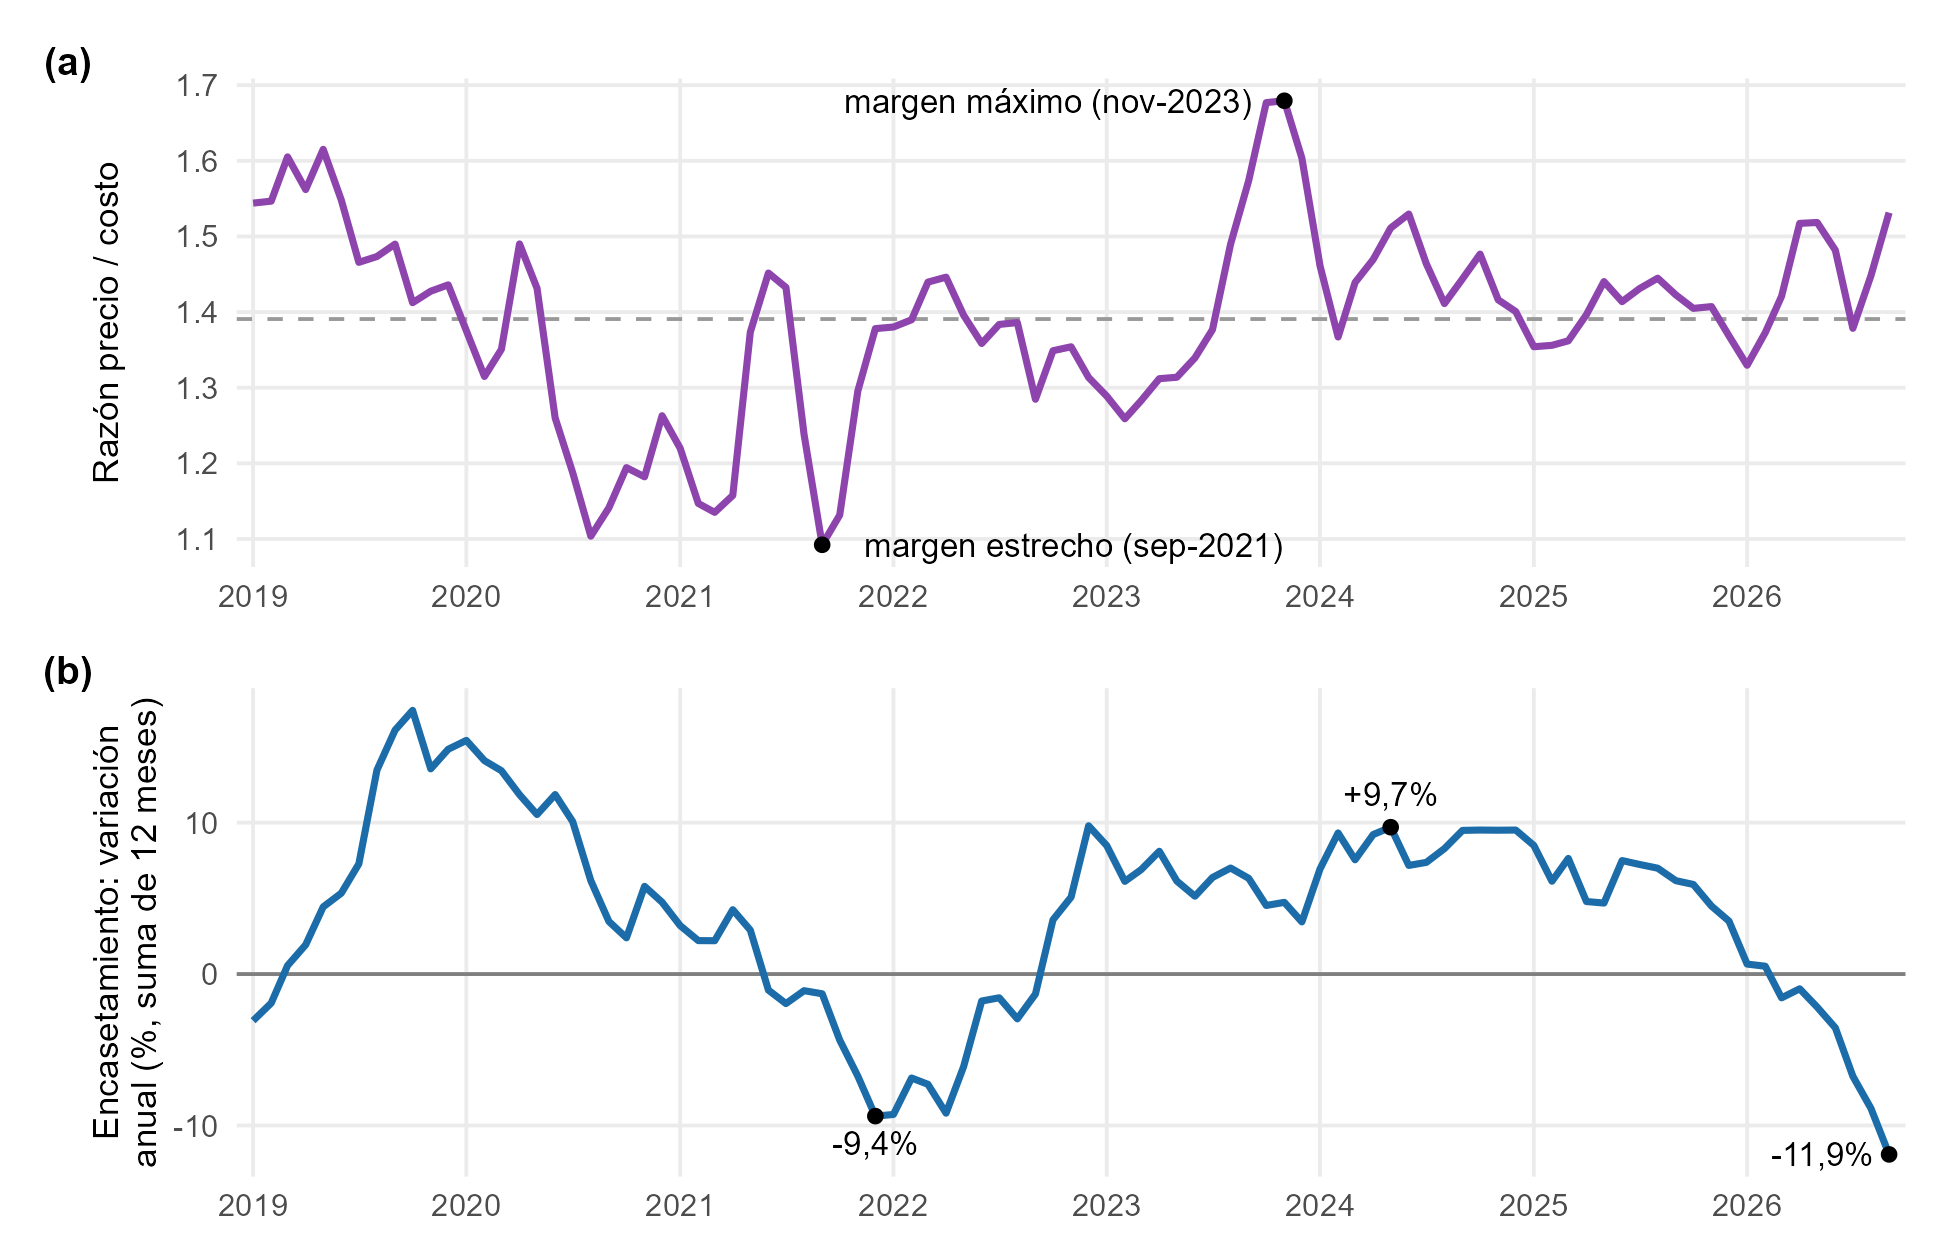
\includegraphics[width=\textwidth]{fig_margen_encasetamiento}
\caption{Margen del productor y decisión de encasetamiento, 2019--2026. (a) Razón entre el precio mayorista del huevo rojo AA y el costo de producción sin amortización del ave; la línea discontinua es su promedio (1,39). (b) Variación anual del encasetamiento (suma de 12 meses). Fuente: elaboración propia con base en \citet{Fenavi2026Estadisticas}, \citet{Fenavi2026Costos} y \citet{DANE2026SIPSA}.}
\label{fig:margen}
\end{figure}

\begin{figure}[!htbp]
\centering
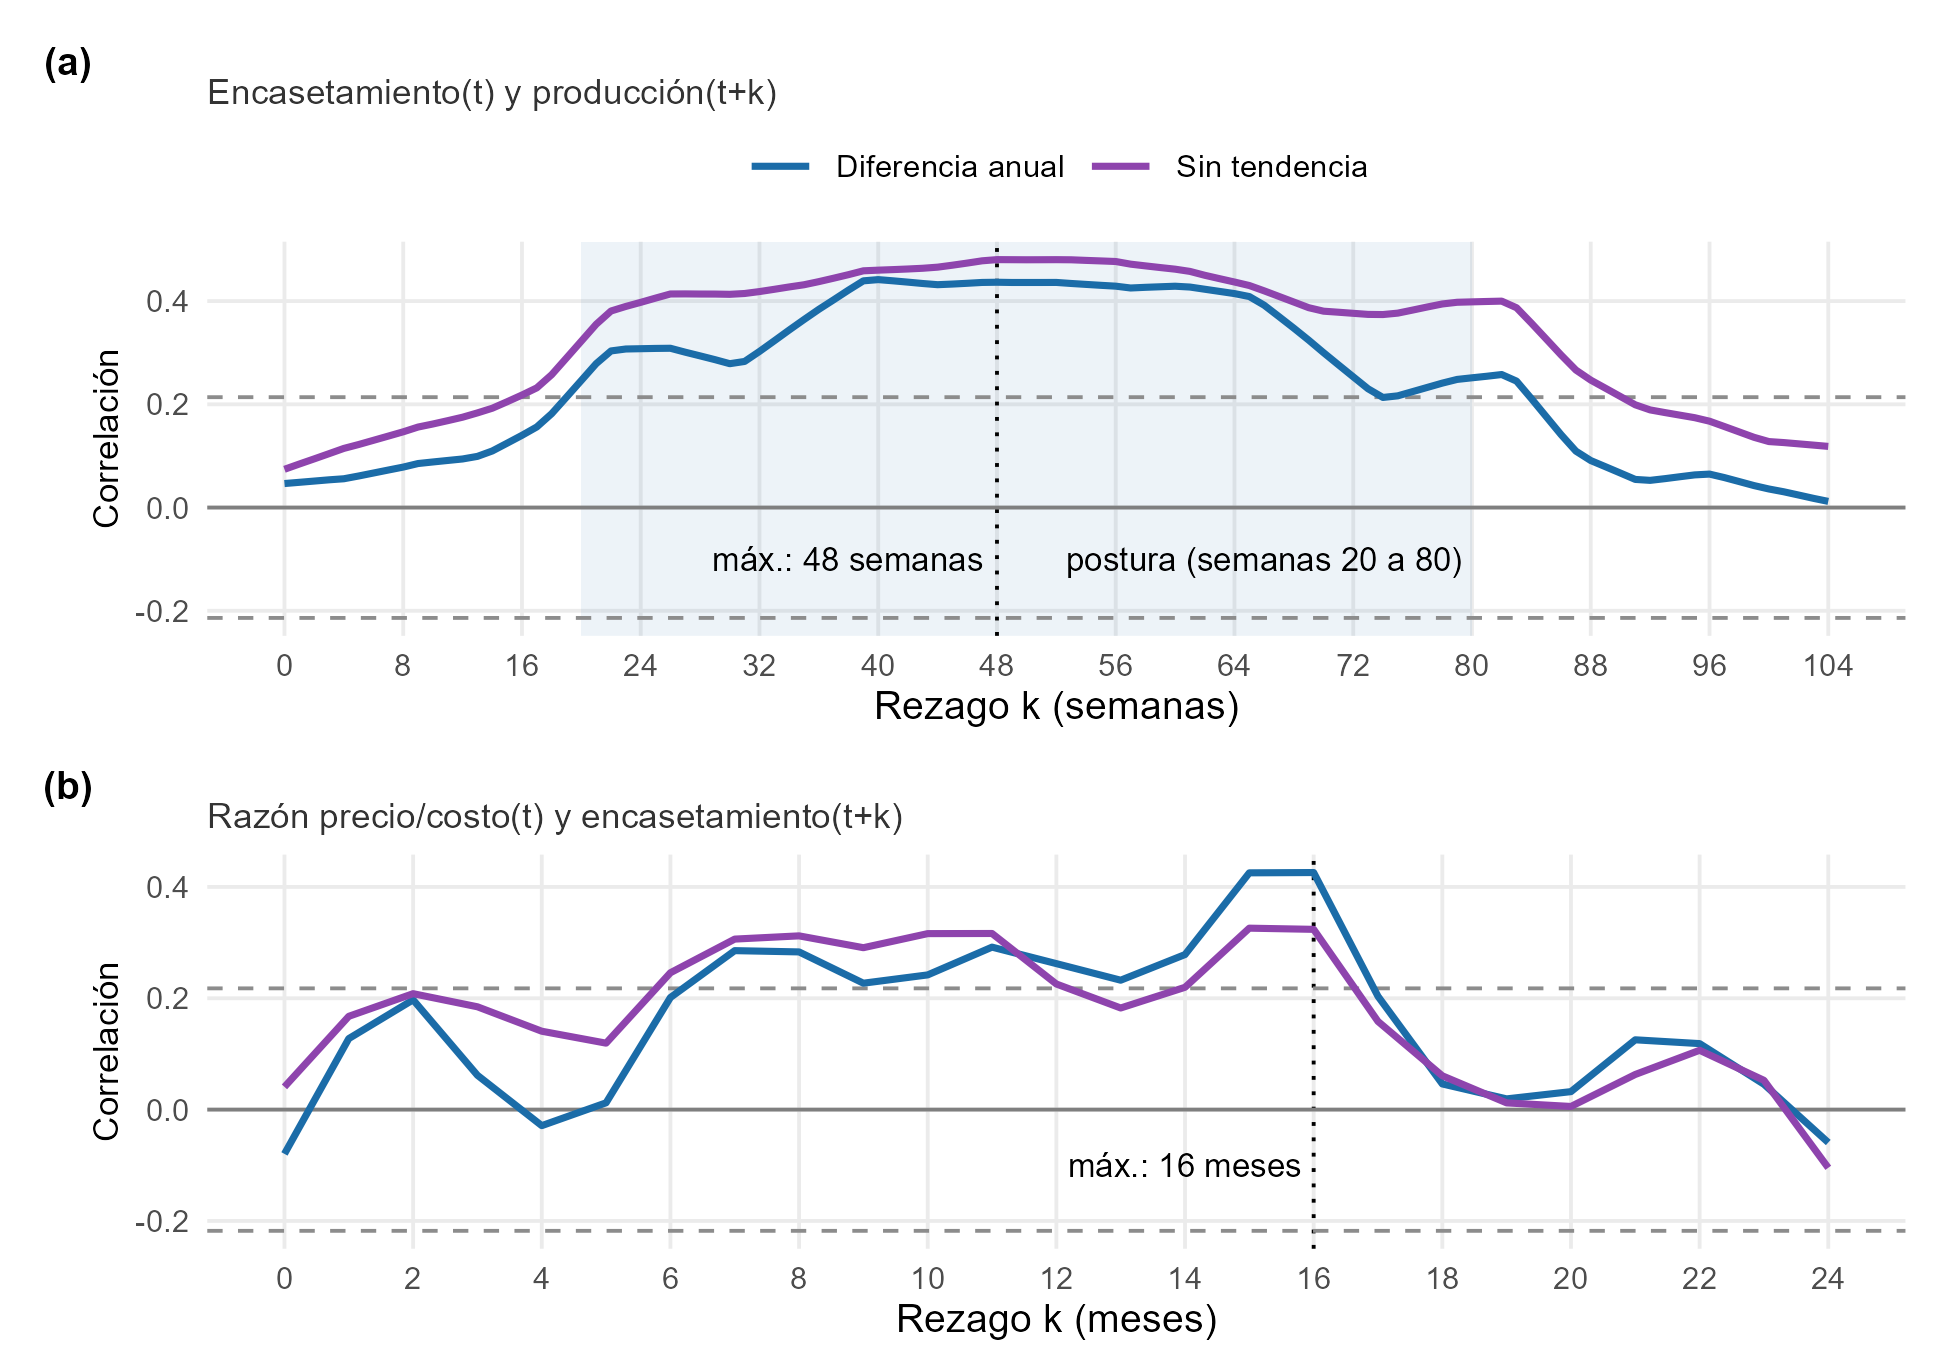
\includegraphics[width=\textwidth]{fig_correlacion_retardos}
\caption{Correlación cruzada de los dos retardos del bucle, con las series en diferencia anual y sin tendencia. (a) Encasetamiento en la semana \textit{t} y producción en la semana \textit{t}~+~\textit{k}; (b) razón precio/costo en el mes \textit{t} y encasetamiento en el mes \textit{t}~+~\textit{k}. Líneas discontinuas: banda de $\pm 1{,}96/\sqrt{n}$ (\textit{n}~=~84 y 81 meses), referencia aproximada que supone ruido blanco. En (a) solo se usa la producción observada, hasta diciembre de 2025. Fuente: elaboración propia con base en \citet{Fenavi2026Estadisticas}, \citet{Fenavi2026Costos} y \citet{DANE2026SIPSA}.}
\label{fig:correlacion}
\end{figure}

Las correlaciones son descriptivas: no prueban causalidad y sus bandas de significancia son aproximadas. Sirven para fijar el orden de magnitud de las demoras que el modelo debe reproducir, y para contrastar después las que resulten de la calibración.

\begin{table}[!htbp]
\centering
\caption{Eslabones del bucle de producción de huevo: retardos y evidencia en los datos.}
\label{tab:eslabones}
\footnotesize
\setlength{\tabcolsep}{4pt}
\begin{tabularx}{\textwidth}{@{}P{2.3cm}P{1.8cm}P{2.1cm}LP{2.0cm}@{}}
\toprule
Eslabón & Mecanismo & Retardo & Evidencia en los datos & Fuente \\
\midrule
Margen $\rightarrow$ encasetamiento & Decisión del productor & 7 a 16 meses (máximo a los 16) & \textit{r}~=~0,43 entre la razón precio/costo y el encasetamiento (variaciones anuales) & Cálculo propio con Fenavi y SIPSA \\
\addlinespace
Encasetamiento $\rightarrow$ inicio de postura & Levante de la pollita & 20 semanas & Supuesto del modelo de población de Fenavi & \citet{Fenavi2026Fenaviquin440} \\
\addlinespace
Encasetamiento $\rightarrow$ producción & Vida productiva del ave & Semanas 20 a 80 (máximo a las 48); 12 meses en variación anual & \textit{r}~=~0,48 (semanal, sin tendencia); \textit{r}~=~0,94 (variaciones anuales) & Cálculo propio con Fenavi \\
\addlinespace
Producción $\rightarrow$ precio & Mercado & Sin rezago & \textit{r}~=~$-$0,60 (semanal, sin tendencia); \textit{r}~=~$-$0,59 entre la brecha de producción por habitante y la del precio & Cálculo propio con Fenavi, SIPSA y DANE \\
\addlinespace
Precio $\rightarrow$ margen & Ingreso frente al costo & Inmediato & La razón usa el precio del mismo mes; el costo depende del maíz, la soya y la TRM (exógenos) & Fenavi; SIPSA \\
\bottomrule
\end{tabularx}

\smallskip
{\footnotesize\raggedright Bucle de balance con retardos: margen alto $\rightarrow$ más encasetamiento $\rightarrow$ (levante y postura) $\rightarrow$ más producción $\rightarrow$ precio más bajo $\rightarrow$ margen más bajo. Fuente: elaboración propia.\par}
\end{table}

\subsubsection{Causa sistémica del problema}

Con la formulación, la descripción del sistema y la evidencia de los retardos, la causa del problema se define en términos de la estructura, como proponen \citet{RubianoVillarreal}:

\medskip
\noindent \textit{La estructura de la cadena del huevo en Colombia combina una regla de encasetamiento que responde al margen percibido y descuenta solo una parte de las aves en levante, dos demoras biológicas largas, una demanda poco sensible al precio y una capacidad de galpones que crece en las bonanzas y casi no se retira en las crisis. Esa estructura genera por sí misma la alternancia de sobreoferta y escasez, aun sin choques externos.}

\medskip
Esta es la hipótesis dinámica que el modelo pone a prueba. Coincide con la estructura de los ciclos de commodities que describe \citet{Sterman2000}, en la que el ciclo surge de bucles de balance que actúan con demoras distintas: la respuesta de la demanda al precio, el uso de la capacidad existente y la construcción de capacidad nueva.

%% -------------------------------------------------------------------
\subsection{Mapa del problema}
\label{sec3.5}

La Figura~\ref{fig:mapa} presenta el mapa del problema con la forma que proponen \citet{RubianoVillarreal}. A la izquierda están los parámetros de definición de escenarios. Cuatro son políticas que el sector o el Estado pueden adoptar, y todas se activan en enero de 2027:
\begin{itemize}
\item \textit{Información completa}: la fracción de la línea de suministro que considera el productor pasa de 0,34 \citep{Sterman1989b} a 1, como si el encasetamiento de todo el sector se conociera a tiempo.
\item \textit{Cuota de encasetamiento}: el encasetamiento se limita a 1.078.000 pollitas por semana, el que repone la producción de 2025, cuando la caja del productor cae por debajo del 30~\% de su nivel de referencia.
\item \textit{Fondo de estabilización}: compra hasta 50 millones de huevos por semana, cerca del 13~\% de la producción de 2025, cuando el precio en granja cae por debajo del costo total del productor; la compra crece con la diferencia entre los dos.
\item \textit{Vida productiva más larga}: la vida productiva normal de las gallinas pasa de 60 a 71 semanas, el óptimo económico de \citet{TraoreDoyon2023}.
\end{itemize}
%% PENDIENTE (modelo v3): la caja relativa del modelo toma valores de -118 a +38,
%% así que el umbral de 0,3 de la cuota hay que redefinirlo antes de correr ese
%% escenario (ver Cambios_modelo_v3.md, punto 7.5). Ajustar este texto si cambia.

Los otros dos parámetros son choques que nadie controla y que sirven para probar qué tan robusta es cada política: un alza de 15~\% en el precio del maíz y la torta de soya desde enero de 2027, y un brote de influenza aviar que, desde finales de marzo de 2027, saca el 10~\% de las gallinas durante 18 semanas; esas magnitudes se tomaron del brote H7N3 de los Altos de Jalisco (México) en 2012 \citep{SENASICA2022}.

A la derecha están los indicadores, que se miden entre enero de 2027 y diciembre de 2030, la ventana en que actúan las políticas: las semanas con margen negativo y los productores que salen miden el efecto sobre el productor; el coeficiente de variación del precio real, la estabilidad del mercado; y el precio real medio y el consumo aparente por persona, el efecto sobre los hogares. Cada parámetro y cada indicador es una variable del modelo, así que un escenario se define al cambiar un valor o activar un interruptor.

%% ---- Mapa del problema dibujado con TikZ ----
%% Se dibujó en LaTeX para que el texto se pueda corregir aquí mismo.
%% Si prefieren la imagen del borrador (figuras/mapa_problema_borrador.png),
%% actualícenla primero (horizonte 2019-2030, choques desde 2027, indicadores
%% medidos en 2027-2030) y cambien todo el tikzpicture por:
%%   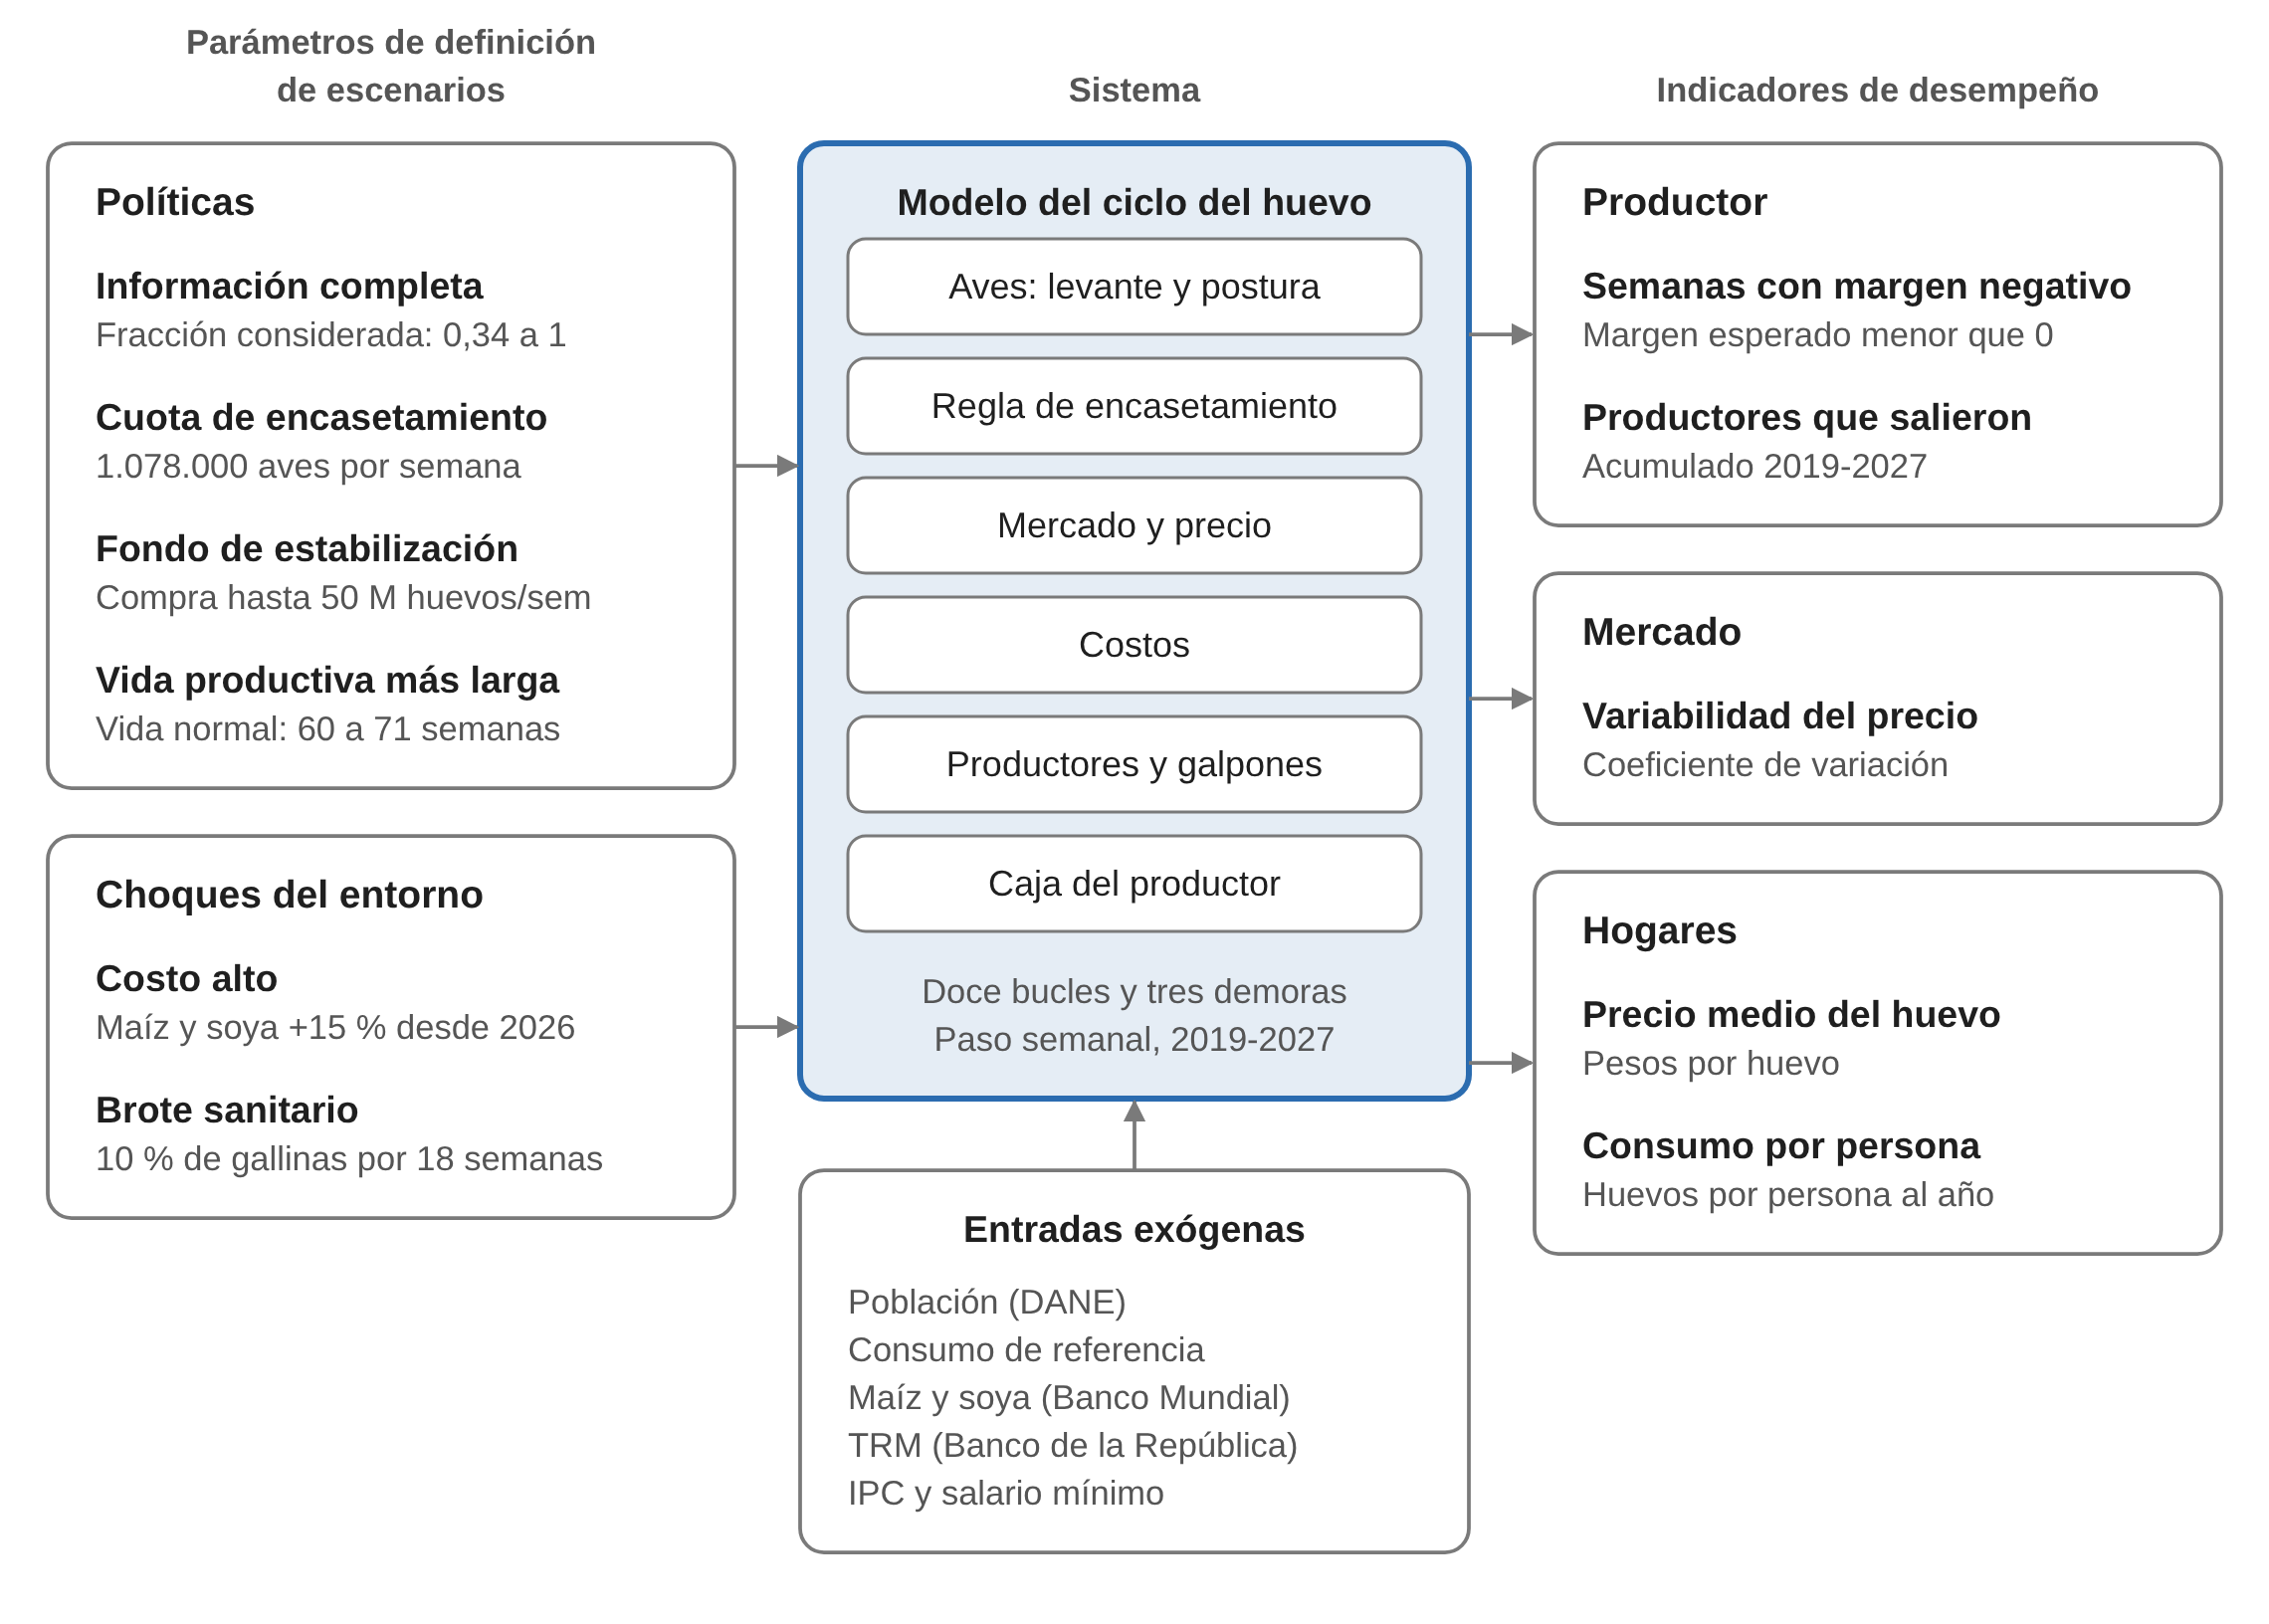
\includegraphics[width=\textwidth]{mapa_problema_borrador}
\begin{figure}[!htbp]
\centering
\begin{tikzpicture}[
  font=\sffamily\scriptsize,
  caja/.style={draw=black!45, rounded corners=3pt, line width=0.6pt,
               align=left, inner sep=3.5pt, text width=3.85cm},
  sector/.style={draw=black!40, fill=white, rounded corners=2pt,
                 text width=3.25cm, align=center, minimum height=5mm},
  encabezado/.style={font=\sffamily\footnotesize\bfseries, text=black!65,
                     align=center, text width=3.9cm},
  titulocaja/.style={font=\sffamily\footnotesize\bfseries},
  flecha/.style={-{Stealth[length=2.2mm]}, draw=black!60, line width=0.8pt}
]
%% Encabezados de las tres columnas
\node[encabezado, anchor=south] at (2.05,0.15) {Parámetros de definición\\de escenarios};
\node[encabezado, anchor=south] at (6.85,0.15) {Sistema};
\node[encabezado, anchor=south] at (11.65,0.15) {Indicadores de desempeño\\(2027--2030)};

%% Izquierda: políticas y choques
\node[caja, anchor=north west] (pol) at (0,0) {%
  {\titulocaja Políticas}\\[3pt]
  \textbf{Información completa}\\ fracción considerada de la línea de suministro: de 0,34 a 1\\[3pt]
  \textbf{Cuota de encasetamiento}\\ 1.078.000 pollitas por semana cuando la caja cae bajo el 30~\% de su referencia\\[3pt]
  \textbf{Fondo de estabilización}\\ compra hasta 50 millones de huevos por semana si el precio en granja no cubre el costo\\[3pt]
  \textbf{Vida productiva más larga}\\ de 60 a 71 semanas};
\node[caja, anchor=north west] (cho) at ([yshift=-4mm]pol.south west) {%
  {\titulocaja Choques del entorno}\\[3pt]
  \textbf{Costo alto}\\ maíz y torta de soya 15~\% más caros\\[3pt]
  \textbf{Brote sanitario}\\ sale el 10~\% de las gallinas durante 18 semanas};

%% Centro: el modelo y sus seis sectores
\node[titulocaja] (tmod) at (6.85,-0.35) {Modelo del ciclo del huevo};
\node[sector, below=2.5mm of tmod] (s1) {Aves: levante y postura};
\node[sector, below=1.5mm of s1] (s2) {Regla de encasetamiento};
\node[sector, below=1.5mm of s2] (s3) {Mercado y precio};
\node[sector, below=1.5mm of s3] (s4) {Costos};
\node[sector, below=1.5mm of s4] (s5) {Productores y galpones};
\node[sector, below=1.5mm of s5] (s6) {Caja del productor};
\node[below=2mm of s6, align=center, text width=3.3cm, text=black!70] (nota)
  {Paso semanal, 2019--2030\\ políticas y choques desde enero de 2027};
\begin{scope}[on background layer]
\node[fit=(tmod)(s1)(s6)(nota), draw=blue!55!black, fill=blue!6,
      line width=1pt, rounded corners=4pt, inner sep=5pt] (sis) {};
\end{scope}

%% Entradas exógenas, debajo del modelo
\node[caja, anchor=north] (exo) at ([yshift=-6mm]sis.south) {%
  {\titulocaja Entradas exógenas}\\[3pt]
  población (DANE)\\ consumo de referencia\\ maíz y torta de soya (Banco Mundial)\\
  TRM y salario mínimo (Banco de la República)\\ IPC (DANE)};

%% Derecha: indicadores
\node[caja, anchor=north west] (ip) at (9.6,0) {%
  {\titulocaja Productor}\\[3pt]
  \textbf{Semanas con margen}\\\textbf{negativo}: margen esperado menor que cero\\[3pt]
  \textbf{Productores que salen}\\ acumulado en la ventana};
\node[caja, anchor=north west] (im) at ([yshift=-4mm]ip.south west) {%
  {\titulocaja Mercado}\\[3pt]
  \textbf{Variabilidad del precio}\\ coeficiente de variación del precio real};
\node[caja, anchor=north west] (ih) at ([yshift=-4mm]im.south west) {%
  {\titulocaja Hogares}\\[3pt]
  \textbf{Precio medio}\\ precio real promedio\\[3pt]
  \textbf{Consumo por persona}\\ huevos por persona al año};

%% Flechas
\draw[flecha] (pol.east) -- (pol.east -| sis.west);
\draw[flecha] (cho.east) -- (cho.east -| sis.west);
\draw[flecha] (exo.north) -- (sis.south);
\draw[flecha] (ip.west -| sis.east) -- (ip.west);
\draw[flecha] (im.west -| sis.east) -- (im.west);
\draw[flecha] (ih.west -| sis.east) -- (ih.west);
\end{tikzpicture}
\caption{Mapa del problema: parámetros de definición de escenarios, modelo con sus entradas exógenas e indicadores de desempeño. Fuente: elaboración propia con base en \citet{RubianoVillarreal}.}
\label{fig:mapa}
\end{figure}

%% ===================================================================
%% Siguen: 3.6 Hipótesis dinámica, 3.7 Modelo de niveles y flujos,
%% 3.8 Configuración de la simulación, 3.9 Validación, 3.10 Escenarios.

%% Mientras no estén las secciones 3.6 a 6, \clearpage obliga a LaTeX a poner
%% aquí las figuras pendientes, antes de las referencias. Quitarlo después.
\clearpage

%% ===================================================================
%% Estilo autor-año de Elsevier con "y" en lugar de "and" (archivo incluido).
%% Para enviar a la revista en inglés, volver a elsarticle-harv.
\bibliographystyle{elsarticle-harv-es}
\bibliography{referencias}

\end{document}

\endinput
